\documentclass[twoside,english]{uiofysmaster}
%\bibliography{references}

\usepackage{array}
\usepackage{booktabs}
\usepackage{float}
\usepackage{scrextend}
\usepackage{amsfonts}
\usepackage{amsmath,amsfonts,amssymb}
\addtokomafont{labelinglabel}{\sffamily}

\usepackage[boxed]{algorithm2e}
\addtokomafont{labelinglabel}{\sffamily}

% Feynman diagrams
\usepackage[compat=1.1.0]{tikz-feynman}
\usepackage{tikz}

% Feynman slash
\usepackage{slashed}

% To show code
\usepackage{listings}

\setlength{\heavyrulewidth}{1.5pt}
\setlength{\abovetopsep}{4pt}

\usepackage[boxed]{algorithm2e}
\addtokomafont{labelinglabel}{\sffamily}

% Multicolumns for calculation
\usepackage{multicol}

% Subfigures
\usepackage{subcaption}
\usepackage{sidecap}

% For quotes
\usepackage[autostyle]{csquotes} 



\begin{document}


\title{The dings that will become a thesis at some point}
\author{Ingrid Holm}
\date{February 2018}

\maketitle

\begin{abstract}
This is an abstract text.
\end{abstract}

\begin{dedication}
  To someone
  \\\vspace{12pt}
  This is a dedication to my cat.
\end{dedication}

\begin{acknowledgements}
  I acknowledge my acknowledgements.
\end{acknowledgements}

\tableofcontents


\chapter{Introduction}

- why nlo?

- why gp?

- why dgp?


\chapter{Gaussian Processes}

In this chapter Gaussian process regression is introduced. First, some concepts and expressions in Bayesian statistics are reviewed. The following section introduces the mathematical framework needed for Gaussian processes, before selected covariance functions are discussed. Concepts in Bayesian model selection are used as a basis to quantify and improve the quality of predictions. Finally, distributed Gaussian processes are introduced as a way of scaling Gaussian processes to larger datasets.

\section{Introduction to Bayesian Statistics}

There are two general philosophies in statistics, namely \textit{frequentist} and \textit{Bayesian} statistics. To understand where they differ, consider a statement statisticians from both branches consider to be true

\begin{center}
\textit{Statisticians use probability to describe uncertainty.}
\end{center}

The difference between Bayesian and frequentist statistics is at the definition of the \textit{uncertain}. Since uncertainty is described by probability this must also vary, and one distinguishes between \textit{objective} and \textit{subjective} probability. Consider an example in which a statistician throws a dice. Before throwing, he is uncertain about the outcome of the dice toss. This uncertainty related to the outcome is \textit{objective}: no one can know if he will throw a 1 or a 4. On the other hand, he might also be uncertain about the underlying probability distribution of the dice toss. Is the dice loaded? Is one of the edges sharper than the others? This uncertainty is \textit{subjective}, as it may vary depending on how much information is available about the system. One of the main critiques of subjective probability posed by frequentists is that the final probability depends on who you ask.

\subsection{Bayes' Theorem}

To further illustrate the difference between frequentist and Bayesian statistics \textit{Bayes' theorem} is introduced. Bayes' theorem can be derived from the familiar rules of probability
\begin{align}\label{Eq:: Sum rule}
P(X | I) + P(\bar{X} | I) = 1,
\end{align}
\begin{align}\label{Eq:: Product rule}
P(X, Y | I) = P(X | Y, I) \times P(Y | I),
\end{align} 
commonly known as the \textit{sum rule} and \textit{product rule}, respectively. $P(X|I)$ is the probability of outcome $X$ given the information $I$, and $P(X|Y,I)$ is the probability of outcome $X$ given the information $I$ \textit{and} outcome $Y$. The bar over $\bar{X}$ means that the outcome $X$ does \textit{not} happen. The sum rule states that the total probability of the outcomes $X$ and $\bar{X}$ is equal to 1. This is rather untuitive, considering an event either takes place not. The second rule, the product rule, states that the probability of both outcomes $X$ and $Y$ is equal to the probability of $Y$ times the probability of $X$ given that $Y$ has ocurred. These expressions combine to give Bayes' theorem, first formulated by reverend Thomas Bayes in 1763,
\begin{align}\label{Eq:: gaussian process : Bayes theorem}
P(X | Y, I) = \frac{P(Y | X, I) \times P(X | I)}{P(Y | I)}.
\end{align}
This theorem states that the probability of $X$ given $Y$ equals the probability of $Y$ given $X$ times the probability of $X$, divided by the probability of $Y$. Surprisingly, there is nothing Bayesian about Bayes' theorem. It merely reformulates the rules of logical consistent reasoning stated by Richard Cox in 1946 \cite{sivia2006data}. Laplace was the one to make Bayes' theorem Bayesian, when he used the theorem to perform inference about distribution parameters. These are, for example, the mean and variance of a Gaussian distribution. The resulting expression is
\begin{align}
P(\Theta = \theta | X=x) = \frac{P(X=x|\Theta = \theta) P(\Theta = \theta)}{P(X=x)},\label{Eq:: gaussian process : Bayesian inference}
\end{align}
where $\Theta$ are the possible probability distribution parameters, $X$ are the possible outcomes, $P(X=x)$ is a normalization constant called the \textit{marginal likelihood}, and $P(X=x|\Theta = \theta)$  and $P(\Theta = \theta)$ are the \textit{likelihood} and \textit{prior}, respectively. In other words, Eq.\ (\ref{Eq:: gaussian process : Bayesian inference}) states the probability of the parameters $\theta$ given the knowledge of outcomes $x$.

A crucial parting of Bayesian statistics from frequentist statistics is at the introduction of the \textit{prior}, which expresses a probability distribution on the \textit{parameters} of the probability distribution.

\subsection{Priors and Likelihood}

The likelihood $P(X = x |\Theta = \theta)$ is simply the probability of the observations $x$ given the parameters of the probability distribution $\theta$. Conversely, the prior expresses a prior belief or assumption of the data, and has to be determined beforehand. The measure $P(\Theta = \theta | X = x)$ from Eq. (\ref{Eq:: gaussian process : Bayesian inference}) is called the \textit{posterior distribution}. This can be thought of as the prior belief, modified by how well this belief fits the data,
\begin{align*}
\text{posterior} = \frac{\text{prior} \times \text{likelihood}}{\text{marginal likelihood}}.
\end{align*}
Consider an example. The statistician from before now sets about tossing a coin. Before tossing he assumes the probability of all outcomes is equal, and so adopts a flat prior probability distribution. After one throw he gets heads, and the posterior changes to a function with high probability for heads, and low for tails. After 4 throws where two were heads and two were tails the posterior shows an equal probabilty for heads and tails, with a wide distribution centered at 0.5. After several throws the distribution converges to a narrow peak around $0.25$, illustrated in Fig.\ (\ref{Fig:: gaussian process : Dice throw }). This indicates an unfair coin that is biased towards tails.

\begin{figure}
\includegraphics[scale=0.85]{figures_gaussian_processes/coin_toss_xd.pdf}
\caption{The posterior probability distribution of the bias-weighting of a coin for the uniform prior, $P(H|I)$. The first panel from the left is before the coin is tossed, the second panel is after 1 toss, the third is after 4 tosses, and the fourth is after 1024 tosses. The posterior converges towards a narrow peak at $0.25$, so the coin is biased.}
\label{Fig:: gaussian process : Dice throw }
\end{figure}


\subsection{Best Estimate and Reliability}

Given a posterior distribution it is important to decide how well it fits the data. For that purpose the \textit{best estimate} and \textit{reliability} are defined. The best estimate $X_0$  is the outcome with the highest probability. In other words, it is the maximum of the posterior
\begin{align}
&\frac{dP}{dX}\Big|_{X_0} = 0, &\frac{d^2P}{dX^2}\Big|_{X_0} < 0.
\end{align}
The second derivative must be negative to insure that $X_0$ is, in fact, a maximum. Equally important to finding a best estimate is knowing how reliable the estimate is. Reliability is connected the width of the distribution, or how much the data is smeared out. A narrow distribution has low uncertainty, while a wide distribution has large uncertainty. The width is found by Taylor expanding the posterior, and taking the logarithm \footnote{$L$ is a monotonic function of $P$, so the maximum of $L$ is at the maximum of $P$.}
\begin{align}
&L = L(X_0) + \frac{1}{2} \frac{d^2}{dx^2} L\Big|_{X_0} (X-X_0)^2 +... ,&L = \log_e \Big[\text{prob}(x | \{data\}, I) \Big]\label{Eq:: gaussian process : Taylor expansion L}
\end{align}
This gives an approximate posterior in the shape of a \textit{Gaussian distribution}, with mean and variance given by
\begin{align}
&\mathcal{N}( \mu, \sigma) \text{ where } \mu = X_0\text{, } \sigma = \Big( - \frac{d^2L}{dx^2} \Big)^{-1/2}.
\end{align}
The Gaussian distribution is symmetric with respect to the maximum at $x = \mu$, and has a full width at half maximum (FWHM) at around $2.35 \sigma$, as shown in Fig. (\ref{Fig:: gaussian process : Gaussian distribution}).

\begin{figure}
\centering
\includegraphics[scale=1.5]{figures_gaussian_processes/gaussian_distribution_xd.pdf}
\caption{A Gaussian probability distribution. The maximum is at the mean value $\mu$, with a full width at half maximum (FWHM) at around $2.35 \sigma$. Figure from \cite{sivia2006data}.}
\label{Fig:: gaussian process : Gaussian distribution}
\end{figure}

\subsection{Covariance}

Before embarking on Gaussian processes the concept of \textit{covariance} is needed. A more detailed description is found in \cite{sivia2006data}. In many cases the equations are not as simple to solve as in Eq.\ (\ref{Eq:: gaussian process : Taylor expansion L}), as the probability distribution might have several quantities of interest $\{ X_i \}$. In that case, a set of \textit{simultaneous equations} must be solved to get the best estimate
\begin{align}\label{Eq:: gaussian process : Best estimate X_i}
\frac{dP}{dX_i} \Big|_{X_{0j}} =0.
\end{align}
To simplify expressions consider the problem in two dimensions, so that $\{ X_i \} = (X, Y)$. The Taylor expansion of $L$ is then
\begin{align}\label{Eq:: gaussian process : Taylor expansion L_i}
L =& L(X_0, Y_0) + \frac{1}{2} \Big[ \frac{d^2L}{dX^2}  \Big|_{X_0, Y_0}(X-X_0)^2 \nonumber \\
& + \frac{d^2L}{dY^2}  \Big|_{X_0, Y_0}(Y-Y_0)^2 + 2 \frac{d^2L}{dXdY}  \Big|_{X_0, Y_0}(X-X_0)(Y-Y_0) \Big] +...
\end{align}
There are now four partial derivatives, reduced to three using the rules for mixed partial derivatives $\frac{\partial^2}{\partial X \partial Y} = \frac{\partial^2}{\partial Y \partial X}$. Writing the quadratic term of Eq.~\ref{Eq:: gaussian process : Taylor expansion L_i} in matrix form gives
\begin{align}
Q = 
\begin{pmatrix}
X-X_0 & Y -Y_0
\end{pmatrix}
\begin{pmatrix}
A & C\\
C & B
\end{pmatrix}
\begin{pmatrix}
X -X_0\\
Y-Y_0
\end{pmatrix},
\end{align}
where the matrix elements are
\begin{align}
&A = \frac{\partial^2 L}{\partial X^2} \Big|_{X_0, Y_0}, &B = \frac{\partial^2 L}{\partial Y^2} \Big|_{X_0, Y_0}, &&C = \frac{\partial^2 L}{\partial X \partial Y} \Big|_{X_0, Y_0}.
\end{align}
The \textit{variance} is defined as the expectation value of the square of deviations from the mean. In the two-dimensional case this becomes \cite{sivia2006data}
\begin{align}
\text{Var}(X) = \sigma_x^2 = \braket{(X - X_0)^2} = \int \int (X - X_0)^2 P (X, Y | \{\text{data}\}, I) dXdY.
\end{align}
This is the variance $\sigma_X^2$ for $X$, and its square root is the standard deviation $\sigma_X$. A similar expression can be found for $Y$, by switching $X$ and $Y$. It is also possible to find the simultaneous deviations of the parameters $X$ and $Y$, or the correlation between the inferred parameters. This is called the \textit{covariance} $\sigma_{XY}^2$, and is in two dimensions given by
\begin{align}
\sigma_{XY}^2 = \braket{(X - X_0) (Y - Y_0)} =\int \int (X - X_0) (Y - Y_0) P (X, Y | \{\text{data}\}, I) dXdY.
\end{align}
The covariance indicates how an over- or underestimation of one parameter affects another parameter. If, for example, an overestimation of $X$ leads to an overestimation of $Y$, the covariance is positive. If the overestimation of $X$ has little or no effect on the estimation of $Y$, the covariance is negligible or zero $|\sigma_{XY}| \ll \sqrt{\sigma_X^2 \sigma_Y^2}$. These effects are illustrated in Fig.\ (\ref{Fig:: gaussian process : Covariance illustrated}). It can be shown that \cite{sivia2006data}
\begin{align}
\text{cov} = 
\begin{pmatrix}
\sigma_X^2 & \sigma_{XY}^2\\
\sigma_{XY}^2 & \sigma_Y^2
\end{pmatrix}
= - \begin{pmatrix}
A & C\\
C & B
\end{pmatrix}^{-1}.
\end{align}
This is called the \textit{covariance matrix}.

\begin{figure}
\centering
\includegraphics[scale=1.0]{figures_gaussian_processes/covariance_xd.pdf}
\caption{A schematic illustration of covariance and correlation. (a) The contours of a posterior pdf with zero covariance, where the inferred values of $X$ and $Y$ are uncorrelated. (b) The corresponding plot when the covariance is large and negative; $Y + mX =$ constant along the dotted line (where $m > 0$), emphasizing that only this sum of the two parameters can be inferred reliably. (c) The case of positive correlation, where we learn most about the difference $Y − mX$; this is constant along the dotted line.}
\label{Fig:: gaussian process : Covariance illustrated}
\end{figure}


\section{Gaussian Process Regression}

Gaussian processes (GP) is a supervised machine learning method, designed to solve regression and probabilistic classification problems. In this thesis only regression will be used. 

%As experience dictates that Gaussian processes can be hard to grasp, it will serve both the reader and the author well to begin on a conceptual level: \textit{what do Gaussian processes do?}

Consider a set of points $\mathcal{D} = \{\textbf{x}_i, y_i\}$, where $y$ is some (possibly noisy) function of $\textbf{x}$, $y = f(\textbf{x}) + \varepsilon$. This is illustrated by the black dots in in Fig. (\ref{Fig:: gaussian process : GP illustration}). In machine learning $\mathcal{D}$ is the \textit{training data}, as it is used to train the model. It consists of \textit{features}, which are the input vectors $\textbf{x}_i$, and \textit{targets}, which are the function values $y_i$. The set of points is discrete, so there is some $\textbf{x}^*$ for which the target $y^*$ is unknown. Gaussian Processes (GP) predict a Gaussian distribution \textit{over function values} at this point $\textbf{x}^*$, with a corresponding mean $m(\textbf{x}^*)$ and variance $\sigma^2$. The GP prediction for the target value $y^*$ is the mean $m(\textbf{x}^*)$, with uncertainty $\sigma^2$. The predicted target $y^*$ can be viewed as a linear combination of the known targets $y_i$, where the weights are controlled by the covariances between $\textbf{x}_i$ and the test point $\textbf{x}^*$.  


\begin{figure}
\centering
\includegraphics[scale=1.5]{figures_gaussian_processes/gp_illustration_xd.pdf}
\caption{An illustration of a GP prediction of the target value $y^*$ (blue cross), given the known set of points $\{x_i, y_i\}$ (black dots). The prediction is a Gaussian distribution in $y$ with mean $y^*$ and variance $\sigma^2$. The Gaussian distribution is drawn in red with $y$ on the vertical axis, with uncertainty in the $y$-direction.}
\label{Fig:: gaussian process : GP illustration}
\end{figure}

\subsubsection{Function Space View}

Since Gaussian processes provide distributions over functions, it is useful to consider the problem in the function space view introduced in \cite{rasmussen2006gaussian}. For a real process $f(\textbf{x})$ the mean  $m(\textbf{x})$ and covariance function $k(\textbf{x}, \textbf{x}')$ are defined as
\begin{align}
m(\textbf{x}) &= \mathbb{E}[f(\textbf{x})],\\
k(\textbf{x}, \textbf{x}') &= \mathbb{E} [(f(\textbf{x}) - m(\textbf{x}))(f(\textbf{x}') - m(\textbf{x}'))],
\end{align}
where $\mathbb{E}[a]$ is the expectation value of some quantity $a$. Given the mean and covariance, the Gaussian distribution for $f(\textbf{x})$ is completely specified
\begin{align}
f(\textbf{x}) \sim \mathcal{GP}(m(\textbf{x}), k(\textbf{x}, \textbf{x}')).
\end{align}
The covariance between two points $k(\textbf{x}_i, \textbf{x}_j)$ is decided by the \textit{kernel function}. In this text the running example will be the squared exponential (SE) kernel, given by
\begin{align}
k(f(\textbf{x}_i), f(\textbf{x}_j)) = k(\textbf{x}_i, \textbf{x}_j) = \exp \Big( - \frac{1}{2} |\textbf{x}_i - \textbf{x}_j|^2 \Big).
\end{align}
Note that the covariance of the function values $f(\textbf{x}_i)$, $f(\textbf{x}_j)$ only depends on the input parameters $\textbf{x}_i$, $\textbf{x}_j$. 

Specifying the covariance function specifies a distribution over functions \cite{rasmussen2006gaussian}. This is because allowed functions must obey the correlation decided by $k(\textbf{x}_i, \textbf{x}_j)$. Using the kernel on a set of input vectors contained in the matrix $X^*$, gives the \textit{covariance matrix}. Combined with an initial mean of zero \footnote{The mean does not have to be zero, it could for example be the mean of the training data.} one obtains the \textit{prior} distribution
\begin{align}
f(x) \sim \mathcal{N} (0, K(X^*, X^*)).
\end{align} 
This distribution encodes the prior knowledge about the function values $f(x)$, and so the choice of kernel is one of the most important steps in learning with GPs. The prior is modified by the training data to provide a posterior distribution. In Fig.\ (\ref{Fig:: gaussian process : prior posterior drawn samples}) samples are drawn from both the prior and posterior distribution. Samples are here taken to mean functions that obey the covariance function. In the case of the prior, the samples are drawn from a distribution of functions with mean zero and constant variance, meaning that if you drew enough functions the mean value of all functions at every $x$ would be zero. For the posterior, the mean values and uncertainties have been modified by the training data. In a point where there is training data the uncertainty is zero \footnote{Assuming there is no noise in the data.}, and so all samples drawn from this distribution must pass through this point. Far away from training points the uncertainty is large.

\begin{figure}
\centering
\includegraphics[scale=0.55]{figures_gaussian_processes/draw_samples_benchmark.pdf}
\caption{Drawing functions from the prior (top) and posterior (bottom) distributions. The thick, black line represents the mean of the distribution, while the shaded, blue area is the uncertainty. The multiple colored lines are functions drawn randomly from the prior and posterior distributions, whose correlation are dictated by the covariance function. The prior has mean 0 and covariance given by the squared exponential function. The posterior has been modified by training points (red dots), giving rise to zero uncertainty at the points where training data exists, and an altered mean value for the distribution. Figure generated using scikit-learn.}
\label{Fig:: gaussian process : prior posterior drawn samples}
\end{figure}

Consider a simple example of a noise-free set of training points $\{\textbf{x}_i, y_i\}$, so that $y = f(\textbf{x})$. The joint distribution of training outputs $\textbf{f}$ and test outputs $\textbf{f}^*$ according to the prior is then
\begin{align}
\begin{bmatrix}
\textbf{f}\\
\textbf{f}^*
\end{bmatrix}
\sim 
\mathcal{N} \Bigg(
\boldsymbol{0},
\begin{bmatrix}
K(X, X) & K(X, X^*)\\
K(X, X^*) & K(X^*, X^*)
\end{bmatrix}
 \Bigg)
\end{align}
For $n$ training points and $n^*$ test points, $K(X,X)$ is the $n \times n$ matrix containing the covariance of training points, $K(X, X^*)$ is the $n \times n^*$ matrix of covariance between the test and training points, and $K(X^*, X^*)$ is the $n^* \times n^*$ matrix containing the covariance of test points. By conditioning the distribution of $\textbf{f}^*$ on the observations,  the posterior distribution over $\textbf{f}^*$ is obtained\footnote{For more details, see Appendix A.2 in \cite{rasmussen2006gaussian}.}  \cite{rasmussen2006gaussian} 
\begin{align}
\textbf{f}_* \big| X_*, X, \textbf{f} \sim \mathcal{N}&(K(X_*, X)K(X, X)^{-1} \textbf{f},\\ &K(X_*, X_*) - K(X_*, X)K(X, X)^{-1}K(X, X_*)).
\end{align}

\subsubsection{Gaussian Noise Model}

Noise-free observations are rare. In most cases targets will contain some noise $y = f(\textbf{x}) + \varepsilon$, where the noise $\varepsilon$ is assumed to follow a Gaussian distribution $\varepsilon \sim \mathcal{N}(0, \sigma_n^2)$. This is the \textit{Gaussian noise model}. The covariance can then be expressed as
\begin{align}
&\text{cov}(y_i, y_j) = k(\textbf{x}_i, \textbf{x}_j) + \sigma_n^2 \delta_{ij} 
\end{align}
which gives for the prior distribution
\begin{align}
\begin{bmatrix}
\textbf{y}\\
\textbf{f}^*
\end{bmatrix}
\sim 
\mathcal{N} \Bigg(
\boldsymbol{0},
\begin{bmatrix}
K(X, X) + \sigma_n^2 \mathbb{I} & K(X, X^*)\\
K(X, X^*) & K(X^*, X^*)
\end{bmatrix}
 \Bigg).
\end{align}
The conditioned distribution is then 
\begin{align}
\textbf{f}^* \big| X^*, X, \textbf{f} & \sim \mathcal{N}(\bar{\textbf{f}}^*, \text{cov}(\textbf{f}^*)), \text{ where} \\
\bar{\textbf{f}}^* &= K(X^*, X) [K(X, X) + \sigma_n^2 \mathbb{I}]^{-1} \textbf{y},\\
\text{cov} (\textbf{f}^*) &= K(X^*, X^*) - K(X^*, X)[K(X, X) + \sigma_n^2 \mathbb{I}]^{-1} K(X, X^*) 
\end{align}

For the sake of tidying up the expression define the matrix $K \equiv K(X, X)$ and the matrix $K^* \equiv K(X, X^*)$. In the case of a single test point $\textbf{x}^*$ the matrix $K^*$ is written as a vector $\textbf{k}(\textbf{x}^*) = \textbf{k}^*$. Using this compact notation the GP prediction for a single test point $\textbf{x}^*$ is
\begin{align}
\bar{f}^* &= \textbf{k}^{*T}(K + \sigma_n^2\mathbb{I})^{-1} \textbf{y},\label{Eq:: gaussian process : GP prediction mean}\\
\mathbb{V}[f^*] &= k(\textbf{x}^*, \textbf{x}^*) - \textbf{k}^{*T}(K + \sigma_n^2 \mathbb{I})^{-1} \textbf{k}^*\label{Eq:: gaussian process : GP prediction variance}.
\end{align}
Note that the predicted mean value $\bar{f}^*$ can be viewed as a linear combination of $y_i$ of the form $\alpha \textbf{y}$, where $\alpha = \textbf{k}^{*T}(K + \sigma_n^2\mathbb{I})^{-1}$. $\alpha$ then only contains the covariance between features.

Eqs. (\ref{Eq:: gaussian process : GP prediction mean})-(\ref{Eq:: gaussian process : GP prediction variance}) form the basis for GP prediction in \verb|scikit-learn|  \cite{scikit-learn}. The algorithm is shown in Algorithm (\ref{Alg:: gaussian process : GP}), and uses the Cholesky decomposition of the covariance matrix.

\begin{algorithm}
\KwData{$X$ (inputs), \textbf{y} (targets), $k$ (covariance function/kernel), $\sigma_n^2$ (noise level), $\textbf{x}_*$ (test input).}
L = Cholesky decomposition ($K + \sigma_n^2 I$) \;
$\boldsymbol{\alpha} = (L^T)^{-1}(L^{-1} \textbf{y})$ \;
$\bar{f}_* = \textbf{k}_*^T \boldsymbol{\alpha}$ \;
$\textbf{v} = L^{-1} \textbf{k}_*$ \;
$\mathbb{V}[f_*] = k(\textbf{x}_*, \textbf{x}_*) - \textbf{v}^T \textbf{v}$ \;
$\log p(\textbf{y}|X) = - \frac{1}{2} \textbf{y}^T \boldsymbol{\alpha} - \sum_i \log L_{ii} - \frac{n}{2} \log 2 \pi$ \;
\KwResult{$f_*$ (mean), $\mathbb{V}[f_*]$ (variance), $\log p(\textbf{y}|X)$ (log marginal likelihood).}
\caption{Algorithm 2.1 from \cite{rasmussen2006gaussian}.}
\label{Alg:: gaussian process : GP}
\end{algorithm}

\section{Covariance Functions}
Covariance functions and kernels have been touched upon, but will be investigated further as they are central to Gaussian processes. A function that only depends on the difference between two points, $\textbf{x} - \textbf{x}'$, is called \textit{stationary}. This implies that the function is invariant to translations in input space. If, in addition, it only depends on the length $r=|\textbf{x}-\textbf{x}'|$, the function is \textit{isotropic} \footnote{Invariant to rigid rotations in input space.}.  Isotropic functions are commonly referred to as \textit{radial basis functions} (RBFs). The covariance function can also depend on the dot product, $\textbf{x} \cdot \textbf{x}'$, and is then called a \textit{dot product} covariance function.

A function which maps two arguments $\textbf{x} \in \mathcal{X}$, $\textbf{x}' \in \mathcal{X}$ into $\mathbb{R}$ is generally called a \textit{kernel} $k$. Covariance functions are symmetric kernels, meaning that $k(\textbf{x}, \textbf{x}') = k(\textbf{x}', \textbf{x})$. As previously mentioned, the matrix containing all the covariance elements is called the \textit{covariance matrix}, or the Gram matrix $K$, whose elements are given by
\begin{align}\label{Eq:: covariance matrix}
K_{ij} = k(\textbf{x}_i, \textbf{x}_j).
\end{align}

The kernel should contain information about the noise in the data, represented by a constant term added to the diagonal
\begin{align}
k(\textbf{x}_i, \textbf{x}_j)_{noise} = C \delta_{ij},
\end{align}
where $C \in \mathbb{R}$ is a real, constant number, and $\delta_{ij}$ is the Dirac delta function. In \verb|scikit-learn| this can be implemented either by giving a fixed noise level $\alpha$ to the regressor function, or by using the \verb|WhiteKernel|, which estimates the noise level from the data. This kernel is implemented in \verb|scikit-learn| in the following way for noise level $0.001$ with bounds $[10^{-10}, 1]$
\begin{lstlisting}
from sklearn.gaussian_processes.kernels import WhiteKernel
whitenoise = WhiteKernel(noise_level=0.001, noise_level_bounds=(1e-10,1))
\end{lstlisting}

\subsection{The Squared Exponential Covariance Function}

The \textit{squared exponential covariance function} (SE) has the form 
\begin{align}
k_{SE} (r) = \exp \Big( - \frac{r^2}{2 \ell^2} \Big),
\end{align} 
where $\ell$ is the \textit{characteristic length scale}. The length scale determines the smoothness of the function. For a large length scale one should expect a very slowly varying function, while a shorter length scale means a more rapidly varying function, see the illustration in Fig.\ (\ref{Fig:: gaussian process : ell variation example}). The SE  is infinitely differentiable and therefore very smooth. 

\begin{figure}
\centering
\includegraphics[scale=1.5]{figures_gaussian_processes/length_scales_xd.pdf}
\caption{The effect of varying the length scale $\ell$. A long length scale (blue) gives a smooth, slowly varying function, while a short length scale (red) gives a more staccato, quickly varying function.}
\label{Fig:: gaussian process : ell variation example}
\end{figure}

The SE is implemented in \verb|scikit-learn| under the name radial basis function, and may be called in the following way for length scale $10$, with bounds on the length scale $[0.01, 100]$
\begin{lstlisting}
from sklearn.gaussian_process.kernels import RBF
rbf = RBF(length_scale=10, length_scale_bounds=(1e-2, 1e2))
\end{lstlisting}



\subsection{The Mat\'{e}rn Class }

The \textit{Mat\'{e}rn class of covariance functions} is given by
\begin{align}
k_{Mat\acute{e}rn} (r) = \frac{2^{1- \nu}}{\Gamma (\nu)} \Big( \frac{\sqrt{2 \nu} r	}{\ell} \Big)^{\nu} K_{\nu} \Big( \frac{\sqrt{2 \nu}r}{\ell} \Big),
\end{align}
where $\nu, \ell > 0$, and $K_{\nu}$ is a modified Bessel function. The hyperparameter $\nu$ controls the smoothness of the function, as opposed to the SE kernel which is by definition very smooth. For $\nu \rightarrow \infty$ this becomes the SE kernel. In the case of $\nu$ being half integer, $\nu = p + \frac{1}{2}$, the covariance function is simply the product of an exponential and a polynomial
\begin{align}
k_{\nu=p+\frac{1}{2}} = \exp \Big(- \frac{\sqrt{2 \nu} r	}{\ell} \Big) \frac{\Gamma(p+1)}{\Gamma(2p + 1)} \sum^p_{i=0} \frac{(p+i)!}{i!(p-i)!} \Big( \frac{\sqrt{8 \nu} r	}{\ell} \Big)^{p-i}.
\end{align}
In machine learning the two most common cases are for $\nu = 3/2$ and $\nu = 5/2$
\begin{align}
k_{\nu = 3/2}(r) &=  \Big(1 + \frac{\sqrt{3}r}{\ell} \Big) \exp \Big( -\frac{\sqrt{3}r}{\ell} \Big),\\
k_{\nu = 5/2}(r) &=  \Big(1 + \frac{\sqrt{5}r}{\ell}  + \frac{5r^2}{3 \ell^2}\Big) \exp \Big( -\frac{\sqrt{5}r}{\ell} \Big).
\end{align}

In \verb|scikit-learn| the hyperparameter $\nu$ is fixed, and so not optimized during training. The Mat\'{e}rn kernel is considered more appropriate for physical processes \cite{rasmussen2006gaussian}, and may be called in \verb|scikit-learn| in the following way for length scale 10, length scale bounds $[0.01, 100]$ and $\nu = 3/2$
\begin{lstlisting}
from sklearn.gaussian_process.kernels import Matern
matern = Matern(length_scale=10, length_scale_bounds=(1e-2, 1e2), nu=1.5)
\end{lstlisting}
For values not in $\nu = [0.5, 1.5, 2.5, \infty]$ \verb|scikit-learn| evaluates Bessel functions explicitly, which increases the computational cost by a factor as high as 10.

\subsubsection{Other Kernels}

There are several kernels which are not discussed here. Kernels can be multiplied and summed to form new kernels, making the space of possible kernels infinite. For further details see chapter 4 in \cite{rasmussen2006gaussian}.





\subsubsection{Hyperparameters}

Each kernel has a vector of hyperparameters, \textit{e.g.} $\boldsymbol{\theta} = (\{M\}, \sigma^2_f, \sigma_n^2)$ for the radial basis function (RBF)
\begin{align}
k(\textbf{x}_i, \textbf{x}_j) = \sigma_f^2 \exp (- \frac{1}{2} (\textbf{x}_i - \textbf{x}_j))^T M (\textbf{x}_i - \textbf{x}_j) + \sigma_n^2 \delta_{ij}.
\end{align}
The matrix $M$ can have several forms, amongst them
\begin{align}
&M_1 = \ell^{-2} \mathbb{I} , &M_2 = \text{diag}(\vec{\ell})^{-2}.
\end{align}
Choosing $\vec{\ell}$ to be a vector in stead of a scalar is in many cases useful, especially if the vector of features contain values of different scales, \textit{e.g.} $\textbf{x} = (x_1, x_2)$ where $x_1 \in [0, 1]$ and $x_2 \in [200, 3000]$. The length scale can be set to a vector in \verb|scikit-learn| by giving the \verb|length_scale| parameter as a \verb|numpy| array of the same dimension as the feature vector $\textbf{x}$.



\section{Model Selection}

The choice of kernel and hyperparameters is important for the quality of the GP prediction. Model selection means finding the  kernel and corresponding hyperparameters that best fit the data. This is referred to as \textit{training} in machine learning. In this section Bayesian model selection is quickly overviewed, and the log marginal likelihood and cross validation are considered.

\subsection{Bayesian Model Selection}

A model has a set of model structures $\mathcal{H}_i$, hyperparameters $\boldsymbol{\theta}$ and parameters $\textbf{w}$. Feature selection is done at all levels in a hierarchical way, by finding the  posterior over \textit{parameters}, the posterior over \textit{hyperparameters} and the posterior for the \textit{model}. Here only the posterior over parameters is considered \cite{rasmussen2006gaussian},
\begin{align}
p(\textbf{w}| \textbf{y}, X, \boldsymbol{\theta}, \mathcal{H}_i) = \frac{p(\textbf{y} | X, \textbf{w}, \mathcal{H}_i) p(\textbf{w}|\boldsymbol{\theta}, \mathcal{H}_i)}{p(\textbf{y}|X, \boldsymbol{\theta}, \mathcal{H}_i)},
\end{align}
as it gives rise to the \textit{marginal likelihood} $p(\textbf{y}|X, \boldsymbol{\theta}, \mathcal{H}_i)$, given by 
\begin{align}
&p(\textbf{y}|X, \boldsymbol{\theta}, \mathcal{H}_i) = \int p(\textbf{y} | X, \textbf{w}, \mathcal{H}_i)p(\textbf{w}| \boldsymbol{\theta}, \mathcal{H}_i) d \textbf{w} & \text{(marginal likelihood)}.
\end{align}
Because of the complexity of integrals involved in model selection, it is common to maximize the marginal likelihood with respect to hyperparameters $\vec{\theta}$. This maximization is what distinguishes Bayesian model selection from other model selection schemes, as it incorporates a trade-off between model complexity and model fit. This means that a complex model will allow for several different kinds of models, but each of them will get a low probability. Meanwhile, simple models will only have a few possibilities, but each of these will have a large probability, see Fig.\ (\ref{Fig:: gaussian process : Marginal likelihood Rasmussen}).

\begin{figure}
\centering
\includegraphics[scale=1.5]{figures_gaussian_processes/marginal_likelihood_xd.pdf}
\caption{The marginal likelihood is the probability of the data, given the model. The number of data points $n$ and inputs $X$ are fixed. The horizontal axis represents an idealized set of all possible vectors of targets $\textbf{y}$. Since the marginal likelihood is a probability distribution it must normalize to unity. For a particular set $\textbf{y}'$, indicated by the dashed line, the intermediate model is preferred to the simple and complex ones.}
\label{Fig:: gaussian process : Marginal likelihood Rasmussen}
\end{figure}

%\begin{align}
%p( \boldsymbol{\theta}| \textbf{y}, X, \mathcal{H}_i) = \frac{p(\textbf{y} | X, \boldsymbol{\theta}, \mathcal{H}_i) p(\boldsymbol{\theta}| \mathcal{H}_i)}{p(\textbf{y}|X,  \mathcal{H}_i)}
%\end{align}
%\begin{align}
%p(\mathcal{H}_i| \textbf{y}, X) = \frac{p(\textbf{y} | X, \mathcal{H}_i) p( \mathcal{H}_i)}{p(\textbf{y}|X)}
%\end{align}

\subsection{Log Marginal Likelihood}

Gaussian process regression models with Gaussian noise have the wonderful trait of analytically tractable integrals for the marginal likelihood. The exact expression for the log marginal likelihood \footnote{The logarithm is used as the marginal likelihood varies rapidly.} can be shown to be \cite{rasmussen2006gaussian}
\begin{align}
\log p(\textbf{y}|X, \boldsymbol{\theta}) = - \frac{1}{2} \textbf{y}^T K_y^{-1} \textbf{y} - \frac{1}{2} \log |K_y| - \frac{n}{2} \log 2 \pi.
\end{align}
Each of the terms has an interpretation: $- \frac{1}{2} \textbf{y}^T K_y^{-1} \textbf{y}$ is the only term involving the data, and is therefore the data-fit; $-\frac{1}{2} \log |K_y|$ is the complexity penalty depending only on the covariance function and the inputs; and $- \frac{n}{2} \log 2 \pi$ is a normalization term. The marginal likelihood is conditioned on the hyperparameters of the covariance function $\vec{\theta}$, and the optimal parameters are found by maximizing. This requires the partial derivatives of the log marginal likelihood (LML)
\begin{align}
\frac{\partial}{\partial \theta_j}
 \log p(\textbf{y}|X, \boldsymbol{\theta}) = \frac{1}{2} \textbf{y}^T K^{-1} \frac{\partial K}{\partial \theta_j} K^{-1} \textbf{y} - \frac{1}{2} \text{tr} (K^{-1} \frac{\partial K}{\partial \theta_j}).
\end{align}
Computing the inverse of a matrix, $K^{-1}$, is computationally complex, and for $n$ training points goes as $\mathcal{O}(n^3)$. Once this is done, however, finding the partial derivatives only requires complexity $\mathcal{O}(n^2)$, and so gradient based optimizers are advantageous.

The LML can have several local optima, as seen in Fig. (\ref{Fig:: gaussian process : LML several local optima}). These correspond to different interpretations of the data. The rightmost optima in Fig. (\ref{Fig:: gaussian process : LML several local optima}) for example, favors a small length scale and smaller noise level. This means that it considers little of the data to be noise. The rightmost optimum has a higher noise level, and allows for several large length scales, as it considers most of the data to be noise. Features with very large length scales are considered superfluous, as the function value depends little on them. Because of this type of complication, it might be wise to restart the optimizer a few times during learning.

\begin{figure}
\centering
\includegraphics[scale=0.6]{figures_gaussian_processes/LML_two_local_maxima.pdf}
\caption{A contour plot of the log marginal likelihood with two local optima. The rightmost optima favours a short length scale and low noise, while the leftmost favors a high noise level and therefore several large length scales. Plot generated using scikit-learn.}
\label{Fig:: gaussian process : LML several local optima}
\end{figure}


\subsection{Cross Validation}

%The error of an estimator can be divided into bias, variance and noise. The bias of an estimator is the average error for differing training sets, the variance is a measure of how sensitive the estimator is to varying data, and noise is a property of the data. High bias corresponds to a model that is too simple, i.e. that it considers much of the signal to be noise, while low bias corresponds to a model that is too complicated, i.e. that it fits the data perfectly but does not model the underlying function very well. 

Cross validation is a means of monitoring the performance of a model. In k-fold validation this is done by dividing the data into $k$ subsets and using $k-1$ folds to train the model, and a single fold to validate it. This is repeated $k$ times. Cross-validation requires a loss function, such as the mean relative deviance or the $R^2$ score. The latter is given by 
\begin{align}
R^2 = 1 - \frac{\sum_{i=0}^{N-1} (y_i - \hat{y}_i)^2}{\sum_{i=0}^{N-1} (y_i - \bar{y})^2},
\end{align}
where $\hat{y}_i$ is the predicted value of the $i$th sample, $y_i$ is the true value and $\bar{y} = \frac{1}{N} \sum_{i = 0}^{N-1} y_i$ for $N$ samples. This is the score used for cross validation in this thesis.

Cross-validation can be used to plot learning curves, which is a tool to find out whether the model benefits from adding more data. The learning curve plots the training score and validation score used to find out if the model is \textit{overfitting} or \textit{underfitting}. \textit{Overfitting} means that the model is a perfect fit to the training data, but predicts poorly for test data because it is not general. \textit{Underfitting} occurs when the model is not able to capture the underlying structure of the data. 

Examples of learning curves are shown in Fig.\ (\ref{Fig:: gaussian process : learning curves}) for Naive Bayes and SVM estimators \footnote{Methods in Machine Learning.}. In a) both the training score and cross-validation score tend to a value below 1, which indicates underfitting. This model will not benefit from more data. The example in b) shows a training score of approximately 1, and a cross validation score that converges towards 1. This model could benefit from more data.

\begin{figure}
    \centering
    \begin{subfigure}[b]{0.45\textwidth}
        \includegraphics[width=\textwidth]{figures_gaussian_processes/learningcurve_2.pdf}
        \caption{Underfitting.}
        \label{fig:gull}
    \end{subfigure}
    \begin{subfigure}[b]{0.45\textwidth}
        \includegraphics[width=\textwidth]{figures_gaussian_processes/learningcurve.pdf}
        \caption{Well fit.}
        \label{fig:tiger}
    \end{subfigure}
\caption{Learning curves for two different estimators.}
\label{Fig:: gaussian process : learning curves}
\end{figure}



\subsection{Relative Deviance}

In this project the main loss function used for comparing predictions is the relative deviance. For true values $y_i$ and values predicted by the estimator $\hat{y}_i$ this is given by
\begin{align}
\varepsilon_i = \frac{y_i - \hat{y}_i}{y_i}.
\end{align} 
The relative deviance is used because of the large span of the target values, ranging from about $10^{-30}$ to $10^9$. The data is therefore divided into decades, meaning one set contains $\sigma \in [10^i, 10^{i+1}]$. Then a distribution over the relative deviances within each decade is found, with a mean value and variance. These are plotted as a function of $i$. 

\section{Distributed Gaussian Processes}

\subsubsection{Limitations of Gaussian Processes}

The biggest weakness of Gaussian processes is that they scale poorly with the size of the data set $n$. The training and predicting scale as $\mathcal{O}(n^3)$ and $\mathcal{O}(n^2)$, respectively, giving GP a practical limit of $\mathcal{O}(10^4)$.

In \cite{deisenroth2015distributed} a way of scaling GPs to large data sets is proposed, in the form of a robust Bayesian Comittee Machine (rBCM). This method is based on the product-of-experts and Bayesian Comittee Machine, and has the advantage of providing an uncertainty for the prediction.


\subsection{Product-of-Experts}

Product-of-expert (PoE) models are a way of parallelising large computations. They combine several independent computations on subsets of the total data, called `experts'. In the case of distributed Gaussian processes each expert performs GP on a subset of the training data, and the predictions on a common test set are combined.

Consider the training data set $\mathcal{D} = \{ \textbf{X}, \textbf{y}\}$, which is partitioned into $M$ subsets $\mathcal{D}^{(k)} = \{\textbf{X}^{(k)}, \textbf{y}^{(k)} \}$, $k = 1,...,M$. Each GP expert does learning on its training data set $\mathcal{D}^{(k)}$, then predictions are combined at the parent node. This node could also be considered an expert for a PoE with several layers, see Fig. (\ref{Fig:: gaussian process : DGP illustration of layers}). 

\begin{figure}
\centering
\includegraphics[scale=0.3]{figures_gaussian_processes/product_of_experts.png}
\caption{From \cite{deisenroth2015distributed}.}
\label{Fig:: gaussian process : DGP illustration of layers}
\end{figure}

\subsection{Algorithm}

The marginal likelihood factorizes into the product of $M$ individual terms because of the independence assumption \cite{deisenroth2015distributed}. The LML is then
\begin{align}
\log p(\textbf{y}^{(k)}|\textbf{X}^{(k)}, \boldsymbol{\theta}) = - \frac{1}{2} \textbf{y}^{(k)} (\textbf{K}_{\psi}^{(k)} + \sigma_{\varepsilon}^2 \textbf{I})^{-1}\textbf{y}^{(k)} - \frac{1}{2} \log
 |\textbf{K}_{\psi}^{(k)} + \sigma_{\varepsilon}^2 \textbf{I} |,
\end{align}
where $a^{(k)}$ is the quantity corresponding to the $k$th expert. Computing the LML now entails inverting the $n_k \times n_k$ matrix $(\textbf{K}_{\psi}^{(k)} + \sigma_{\varepsilon}^2 \textbf{I})$, which requires time $\mathcal{O}(n_k^3)$ and memory consumption $\mathcal{O}(n_k^2 + n_kD)$ for $\textbf{x} \in \mathbb{R}^D$. For $n_k \ll N$, this reduces the computation time and memory use considerably, and allows for parallel computing. 

Several methods for prediction are discussed in \cite{deisenroth2015distributed}, but here only the robust Bayesian Comittee Machine is introduced. The PoE predicts a function value $f^*$ at a corresponding test input $\textbf{x}^*$ according to the predictive distribution
\begin{align}
p(f^* | \textbf{x}^*, \mathcal{D}) = \frac{\prod_{k=1}^M p_k^{\beta_k} (f^*| \textbf{x}^*, \mathcal{D}^{(k)})}{p^{-1 + \sum_k \beta_k} (f^* | \textbf{x}^*)}.
\end{align}
This prediction scheme allows for much flexibility, as it can vary the importance of an expert. The combined predictive mean and variance are 
\begin{align}
\mu_*^{rbcm} &= (\sigma_*^{rbcm})^2 \sum_k \beta_k \sigma_k^{-2} (\textbf{x}_*) \mu_k (\textbf{x}_*),\label{Eq:: gaussian process : DGP mu} \\
(\sigma_*^{rbcm})^{-2} &= \sum_{k=1}^M \beta_k \sigma_k^{-2} (\textbf{x}_*) + \big(1 - \sum_{k=1}^M \beta_k \big) \sigma_{**}^{-2},\label{Eq:: gaussian process : DGP sigma}
\end{align}
where the parameters $\beta_k$ control the importance of the individual experts, but also the how strong the influence of the prior is. In the article, these are chosen according to the predictive power of each expert at $\textbf{x}^*$. More specifically, $\beta_k$ is the change in differential entropy between the prior $p(f^* | \textbf{x}^*)$ and the posterior $p(f^* | \textbf{x}^*, \mathcal{D}^{(k)})$, which can be calculated as 
\begin{align}
\beta_k = \frac{1}{2} (\log \sigma_{**}^2 - \log \sigma^2_k(\textbf{x}^*) ),
\end{align}
where $\sigma_{**}^2$ is the prior variance, and $\sigma_k^2 (\textbf{x}^*)$ is the predictive variance of the $k$th expert.


\subsection{Implementing the Algorithm}

The mean and variance in Eq.\ (\ref{Eq:: gaussian process : DGP mu})-(\ref{Eq:: gaussian process : DGP sigma}) were implemented in \verb|Python| using the \verb|scikit-learn| library's existing framework for regular Gaussian processes. The algorithm was parallelised, so that each expert can learn and predict in parallel, before being combined to the final prediction. Pseudocode for the implementation is found in Alg.\ (\ref{Alg:: gaussian process : DGP}).

For parallelisation the \verb|scikit-learn| function \verb|Parallel| from \verb|joblib| was used, which runs Python functions as pipeline jobs. It uses the Python function \verb|multiprocessing| as a backend. An example of usage with 3 parallel jobs is
\begin{lstlisting}
>>> from joblib import Parallel, delayed
>>> from math import sqrt
>>> Parallel(n_jobs=3)(delayed(sqrt)(i**2) for i in range(10))
[0.0, 1.0, 2.0, 3.0, 4.0, 5.0, 6.0, 7.0, 8.0, 9.0]
\end{lstlisting}
where \verb|delayed| is a simple trick to be able to create a tuple with a function-call syntax.


\begin{algorithm}
 \KwData{$N_{experts}$ (number of experts), $X$ (inputs), \textbf{y} (targets), $k$ (initial kernel), $\sigma_n^2$ (noise level), $\textbf{x}^*$ (test input)}
Split training data into $N$ subsets: $X_k, \textbf{y}_k$\;
\For {each expert}
{
Fit GP to training data $X_k, \textbf{y}_k$ \;
 Predict $\mu_*,\sigma_*^2 $ for $\textbf{x}^*$ using GP \;
 $\sigma_{**}^2 = k (x^*, x^*)$ \;
}
 
\For {each expert}
{ 
$\beta = \frac{1}{2} (\log (\sigma_{**}^2) - \log (\sigma_*^2))$ \;
$(\sigma_*^{rbcm})^{-2} += \beta \sigma^{-2} + \big(\frac{1}{n_{experts}} - \beta \big) \sigma_{**}^{-2} $ 
 }  
\For {each expert}
{ 
$\mu_*^{rbcm} += (\sigma_*^{rbcm})^2 \beta \sigma^{-2}_* \mu_*$
} 
\KwResult{Approximative distribution of $f_* = f(\textbf{x}_*)$ with mean $\mu^{rbcm}_*$ and variance $(\sigma^{rbcm}_*)^2$.}
 \caption{Pseudocode for using rBCM on a single test point $\textbf{x}_*$. For the fit and prediction of each expert GP Algorithm (\ref{Alg:: gaussian process : GP}) is used.}
\label{Alg:: gaussian process : DGP}
\end{algorithm}

\subsection{Benchmark}

The benchmark function for parallelised distributed Gaussian processes is
\begin{align*}
f(x_1, x_2) =  4x_1x_2,
\end{align*}
where the vectors $\textbf{x} = (x_1, x_2)$ were drawn from a random normal distribution using the \verb|numpy| function \verb|random.randn|. Gaussian processes implemented by \verb|scikit-learn| in the function \verb|GaussianProcessRegressor| were compared to distributed Gaussian processes with 4 experts. 2000 training points and 1000 test points were used, and the resulting times for the GP and DGP were
\begin{align}
\text{Gaussian processes time: }& 154.12 \text{ s}\\
\text{Distributed Gaussian processes time: }& 5.61 \text{ s}
\end{align}
Histograms of the relative deviances for Gaussian processes (GP) and Distributed Gaussian processes (DGP) are found in Fig.\ (\ref{Fig:: gaussian process : DGP BM error histogram}).

\begin{figure}
\centering
\includegraphics[scale=0.5]{figures_gaussian_processes/DGP_bm_err.pdf}
\caption{Histogram of the relative deviance between true value $y$ and predicted value $\hat{y}$ for Gaussian process regression (GP) and Distributed gaussian process regression (DGP) for the function $f(x_1,x_2) = 4x_1 x_2$.}
\label{Fig:: gaussian process : DGP BM error histogram}
\end{figure}



\chapter{Supersymmetry at Hadron Colliders}

At the moment of writing, the Large Hadron Collider (LHC) at CERN is one of the largest and most important particle physics experiments in the world. In this chapter, some of the advantages and challenges of using hadron colliders are discussed, along with some techniques for moving from theory to physically detectable signals. A short description of supersymmetric phenomenology follows, along with current bounds on some supersymmetric particles. Finally, the squark production cross section is calculated to leading order, and next-to-leading order terms are investigated.

\section{Hadron Colliders}

Colliding hadrons makes it possible to reach very high center-of-mass energies. This is owed to the heavy mass scale of hadrons compared to leptons, resulting in low \textit{synchrotron radiation} which makes the use of circular accelerators beneficial. The circular form means the accelerating structures can be reused as many times as one desires, thus putting `no limits' on the energies obtained (there are, of course, limits). Synchrotron radiation is the radiation of energy from a particle being accelerated, which goes as $\sim m^{-4}$. Thus for light particles, such as the electron, a lot of energy is wasted. The power radiated by a relativistic electron forced to move in circular motion with radius $R$ is given by Schwinger's formula \cite{Balerna2015}
\begin{align}
P_e = \frac{2}{3} \frac{e^2 c}{R^2} \Bigg( \frac{E}{m_e c^2} \Bigg)^4,
\end{align}
where $E$ is the electron energy, $m_e$ is the electron mass and $c$ is the speed of light in vacuum. Because the proton mass is much larger than the electron mass, this effect is relatively small, allowing the LHC to operate at energies currently as high as 13 TeV. 

Amidst this praise of the hadron one question arises: if hadronic colliders are able to reach such high energies, why do bother colliding leptons at all? Alas, the heavy masses come at a kinematical price. The way hadrons are made up of valence and sea quarks and gluons make the kinematics of collisions very difficult to calculate. These quarks and gluons, the so-called \textit{partons}, have the annoying habit of distributing the hadron momentum somewhat randomly amongst themselves. Since we do not know how the energy and momentum is distributed, the momenta of the ingoing particles is unknown. This is why the transverse momentum and energy, not to mention the \textit{missing} transverse energy, are important when analysing data from colliders. However, there is a way to approximate the parton momenta, namely using \textit{parton distribution functions}.

\subsection{Parton Distribution Functions}

Cross sections are calculated for two colliding partons, for example two quarks $q_1 q_2$. The cross section is a function of the center-of-mass energy, $\hat{s}$, which again can be written as a fraction of the center of mass of the colliding protons
\begin{align}
\hat{s} = s x_1 x_2,
\end{align}
where $s$ is the center-of-mass energy of the colliding protons, and $x_i$ is the momentum fraction of the quark $q_i$. The fractions of momenta are then integrated over, using \textit{parton distribution functions} $f(x_i)$, which differ for the different partons. The fraction $x_u$ for an up-type quark in a proton e.g., would be much larger than that for a top-type squark. This yields the total cross section
\begin{align}
\sigma_{q_1q_2} = \int f(x_1) f(x_2) \sigma(\hat{s}) dx_1 dx_2,
\end{align}
where $\sigma$ is the partonic cross section. In this project the CTEQ6 parton distribution functions from the LHAPDF Fortran library \cite{PhysRevD.78.013004} are used.

\subsection{Luminosity}

Another important concept to be introduced is \textit{luminosity}. The luminosity $\mathcal{L}$ is a measure on how many collisions happen at an accelerator per time, and is here given in inverse femto-barn $\text{fb}^{-1} = 10^{43} \text{ m}^{-2}$. This can be used to set limits on the size of cross sections, by considering the following relation for a process where a particle $A$ is produced
\begin{align}
n_{A} = \mathcal{L} \sigma_{A} ,
\end{align}
where $\mathcal{L}$ is the luminosity, $\sigma_{A}$ is the cross section for the production of $A$, and $n_A$ is the number of produced particles. Setting $n=1$ as the limit for a single produced particle, and using $\mathcal{L} = 20.3 \text{ fb}^{-1}$, which is the luminosity for the dataset used here, the lower limit on cross sections is
\begin{align}
\sigma  = \frac{1}{20.3 \text{ fb}^{-1}} \approx 0.05 \text{ fb}.
\end{align}
Therefore, cross sections below $\sigma \sim \mathcal{O}(10^{-3})$, which correspond $0.02$ produced particles, will be less important in this thesis.


\section{Phenomenology}
In order to know what to look for at the LHC it is necessary to consider the phenomenology of supersymmetry. This is done by first revisiting the soft supersymmetry breaking, in order to consider models with more constraints than the 124 parameters of the MSSM. \textit{Hidden sector} (HS) scalar superfields $X$ have very small or no interactions with the MSSM fields. Their couplings are usually supressed by some mass scale so that $\mathcal{L} \sim M^{-1}$. They have an effective (non-renormalizable) interaction  with the scalar superfields of the form
\begin{align}
\mathcal{L}_{HS} &= - \frac{1}{M} (\bar{\theta} \bar{\theta}) X \Phi_i \Phi_j \Phi_k.
\end{align}
If these sectors develope a vacuum expectation value $\braket{X} = \theta \theta\braket{F_X}$ for the auxilliary field $F$ (auxilliary meaning that it can be removed using the Euler-Lagrange equations),  supersymmetry is broken. The two most commonly known hidden sectors are Planck-scale mediated supersymmetry breaking (PMSB) and Gauge mediated supersymmetry breaking (GMSB), the first of which is obtained by blaming some gravity mechanism for mediating the breaking of SUSY from the hidden sector. The breaking scale is then the Plank scale, $M = M_P = 2.4 \cdot 10^{18}$ GeV. The vev is restricted to $\sqrt{\braket{F}} \sim 10^{10} - 10^{11}$ GeV in order not to reintroduce the hierarchy problem.  The complete soft terms can be shown to be \cite{batzing2017lecture}
\begin{align*}
\mathcal{L}_{soft} =& - \frac{\braket{F_X}}{M_P} \Big( \frac{1}{2} f_a \lambda^a \lambda^a + \frac{1}{6} y_{ijk}'A_i A_j A_k + \frac{1}{2} \mu_{ij}' A_i A_j + \frac{\braket{F_X}^*}{M_P^2}  x_{ijk} A_i^* A_j A_k + c.c.\Big)\\
&- \frac{|\braket{F_X}|^2}{M_P} k_{ij}A_i A_j^*.
\end{align*}
By simplifying as much as possible, all soft terms are fixed by just four parameters. This model is called minimal supergravity (mSUGRA) or the constrained minimal supersymmetric Standard Model (CMSSM). The CMSSM parameters are
\begin{align}
&m_{1/2} = f \frac{\braket{F_X}}{M_P}, & m_0^2 = k \frac{|\braket{F_X}|}{M_P^2}, 
&& A_0 = \alpha \frac{\braket{F_X}}{M_P}, &&B_0 = \beta \frac{\braket{F_X}}{M_P},
\end{align}
or $m_{1/2}$, $m_0$, $A_0$, $\tan \beta$ and $\text{sgn} \mu$.

The second hidden sector is the aforementioned Gauge mediated supersymmetry breaking. In this case the soft terms come from loop diagrams with \textit{messenger superfields} that get their own mass from coupling to the HS SUSY breaking vev, and have SM interactions. This model is parameterized by 
\begin{align}
\Lambda = \frac{\braket{F}}{M_{messenger}} \text{ , } M_{messenger} \text{ , } N_5 \text{ , } \tan \beta,
\end{align}
where $M_{messenger}$ is the mass scale and $N_5$ (FYLL INN HER).

\subsection{Searches For Supersymmetry}

Supersymmetry at hadron colliders will be in the form of QCD processes with relatively small masses, as the incoming particles are quarks and gluons and QCD cross sections will therefore be the largest. The traces left by such processes will be closely related to the conservation of $R$-parity, in that all sparticles are produced in pairs and eventually decay to the LSP. If the LSP is indeed only weakly interacting, this makes it very difficult to detect. An indirect way of detecting it, however, is by looking for \textit{missing transverse energy} $\slashed{E}_T$. The energy is only considered in the transverse plane, as the longitudinal momentum is difficult to predict in the hadronic case (see the above discussion of hadron colliders). To look for $\slashed{E}_T$ the \textit{effective mass} is defined as
\begin{align}
M_{eff} &= \sum p_T^{jet} + \slashed{E}_T,
\end{align} 
and used to search for deviations from the SM expectations. Here $p_T^{jet}$ is the transverse momentum of jets. The hadronic jets produced from supersymmetric processes can be very complicated, such as the squark-squark production shown in Fig. (\ref{Fig:: susy hadron : decay at ATLAS}). If all final state particles have low momenta, these are called soft particles. The very large background from SM processes provides another difficulty in searching for supersymmetry. An example generated with ATLAS Open Data is shown in Fig. (\ref{Fig:: susy hadron : ATLAS susy analysis}), where the supersymmetric signals (pink lines) are all below the SM background, and so it is impossible to detect any deviation from SM background. 

\begin{figure}[H]
\centering
\begin{tikzpicture}
\begin{feynman}
\vertex (p1) {\(p\)}; 
\vertex [below right=of p1, blob] (p) {}; 
\vertex [below left=of p] (p2){\(p\)}; 
%----------------------------------
\vertex [right=1.5cm of p] (mid1);\vertex [above=0.7cm of mid1] (s1);
\vertex [below =0.7cm of mid1] (s2);
\vertex [right=1.5cm of s1] (q1); 
\vertex [right=1.5cm of s2] (q2) ; 
%---------------------------------
\vertex [right=1cm of q1] (r1) ; %W
\vertex [right=1cm of q2] (r2) ; %W
%--------------------------------
\vertex [right=1cm of r1] (rl) {\(l\)};
\vertex [above=0.7cm of rl] (rn) {\(\nu\)};
\vertex [right=1cm of r2] (rq1) {\(q\)};
\vertex [below=0.7cm of rq1] (rq2) {\(q\)};
%--------------------------------
\vertex [above=0.7cm of rn] (r11) {\(\tilde{\chi}_1^0\)};
\vertex [below=0.7cm of rq2] (r22) {\(\tilde{\chi}_1^0\)};
\vertex [above=0.7cm of r11] (q11) {\(q\)}; 
\vertex [below=0.7cm of r22] (q22) {\(q\)};
\diagram{
(p1)--(p)--(p2), 
(p) --[scalar, edge label={\(\tilde{q}\)}] (s1), 
(s2) --[scalar, edge label={\(\tilde{q}\)}] (p); 
(q1) --[photon, plain, edge label= {\(\tilde{\chi}_1^{\pm}\)}, ] (s1); 
(s1) -- (q11); (s2) --[photon, plain, edge label= {\(\tilde{\chi}_1^{\pm}\)}] (q2); 
(s2) -- (q22), 
(r1) -- [photon, edge label={\(W\)}] (q1),
 (q1) --[photon, plain](r11), 
 (q2) --[photon, edge label={\(W\)}] (r2), 
 (q2) --[photon, plain] (r22),
(rn)--(r1) -- (rl), 
(rq1) -- (r2) -- (rq2)
};
\end{feynman}
\end{tikzpicture}
\caption{Possible signature of a supersymmetric QCD process, with four quark jets, a lepton and large missing transverse energy in the final state.}
\label{Fig:: susy hadron : decay at ATLAS}
\end{figure}

\begin{figure}
\centering
\includegraphics[scale=0.5]{Figures/mt_rebinned.pdf}
\caption{Analysis of ATLAS data, where the pink lines are supersymmetric signals for $m_{\tilde{q}}=500$ (magenta), $m_{\tilde{q}}=900$ (light pink) and $m_{\tilde{q}}=1100$ (purple). The signal never exceeds the SM background, in this case Diboson (orange), Drell Yan (light blue), $W$ (dark orange), $Z$ (dark blue), $\tilde{t}$ (yellow) and $t \bar{t}$ (green), making it impossible to distinguish events from background. Analysis using $1 \text{ fb}^{-1}$. }
\label{Fig:: susy hadron : ATLAS susy analysis}
\end{figure}

Allowing the violation of R-parity opens up for more possibilities. Then the LSP can decay, and sparticles can be produced one at a time. It is possible to have \textit{massive metastable charged particles} (MMCPs), which are typical for scenarios with a gravitino LSP \cite{batzing2017lecture}.



\subsection{Current Bounds on Sparticles}

Searches and limits are constantly being updated, but here are a few results from the LHC Run I at 8 TeV, with up to $20 \text{ fb}^{-1}$ luminosity. The bounds from the missing energy channel at 8 TeV for mSUGRA from ATLAS are $m_{\tilde{q}} > 1600$ GeV and $m_{\tilde{g}} > 1100$ GeV \cite{batzing2017lecture}.

%\subsection{Precision Observables}

%We can also measure SUSY by considering its impact on very precisey measured SM processes, such as electroweak precision observables, the $(g-2)_{\mu}$ value, the flavour changing neutral current (FCNC) process $b \rightarrow s \gamma$ and the (rare) FCNC process $B_s \rightarrow \mu \mu$.
%
%The electroweak precision observables include $M_W$, $M_Z$, $\Gamma_W$, $\Gamma_Z$, $m_t$ and $\sin \theta_W$, the higgs mass $m_h$ and its properties. Since the Higgs has been measured, we can now do very precise measurements of these quantities, and find that they are very consistent with SM predictions.
%
%The anomalous magnetic moment of the muon, $(g - 2)_{\mu}$, has been measured to extraordinary precision at BNL to be
%\begin{align*}
%g_{\mu} = 2.00116592089(63),
%\end{align*}
%where the digits in parenthesis indicate the uncertainty on the last digits. At tree level we have $\mu \rightarrow \mu \gamma$. Loop corrections to this diagram give $a_{\mu} = (g -2)_{\mu}$. The difference between the SM deviation and the experimentally measured deviation is
%\begin{align*}
%\delta_{a_{\mu}} \equiv a_{\mu}^{exp} - a_{\mu}^{SM}= (25.9 \pm 8.1) \cdot 10^{-10},
%\end{align*}
%which is $3.2 \sigma$ away from zero. This is one of the clearest discrepancies that exist between measurement and the SM.


\section{Squark-Squark Cross Section}
In this thesis the relevant QCD process will be the production of squark pairs in quark-quark collisions,
\begin{align}
q_i q_j \rightarrow \tilde{q}_i \tilde{q}_j,
\end{align}
where $i,j$ are the 4 light quark flavours $u, d, s, c$ which can be equal or different. Top and bottom are not considered here because of their large masses. Feynman diagrams of the leading order for this process can be found in Fig. (\ref{Fig:: susy hadron : Feynman qq}). For equal flavour quarks there are two diagrams contributing: the $t$- and $u$-channel, while for different flavours only the $t$-channel contributes.

\begin{figure}
\centering
\begin{tikzpicture}
\begin{feynman}
\vertex (p1) {\(q_i\)}; \vertex [right= of p1] (s1); \vertex [right= of s1] (q1){\(\tilde{q}_i\)}; \vertex [below=of p1] (p2) {\(q_j\)}; \vertex [right=of p2] (s2) ; \vertex [right= of s2] (q2) {\(\tilde{q}_j\)} ;
\diagram{
(p1) --[fermion, momentum=\(k_1\)] (s1) -- [scalar, momentum=\(p_1\)] (q1), (s1)-- [gluon] (s2) -- (s1), (p2) --[fermion, momentum=\(k_2\)] (s2) --[scalar, momentum=\(p_2\)] (q2)
};
\end{feynman}
\end{tikzpicture}
\begin{tikzpicture}
\begin{feynman}
\vertex (p1) {\(q_i\)}; \vertex [right= of p1] (s1); \vertex [right= of s1] (q1){\(\tilde{q}_i\)}; \vertex [below=of p1] (p2) {\(q_j\)}; \vertex [right=of p2] (s2) ; \vertex [right= of s2] (q2) {\(\tilde{q}_j\)} ;
\diagram{
(p1) --[fermion] (s1) -- [scalar] (q2), (s1)-- [gluon] (s2) -- (s1), (p2) --[fermion] (s2) --[scalar] (q1)
};
\end{feynman}
\end{tikzpicture}
\caption{Feynman diagrams for squark pair production in quark quark collisions, both $t$ and $u$ diagram. Note that the u-channel (right diagram) is only possible for $i=j$.}
\label{Fig:: susy hadron : Feynman qq}
\end{figure}


%\subsection{Feynman Diagrams}

\subsection{Calculation to LO}

The cross section for squark production is here calculated to leading order. The momentum of the gluino is denoted $p$ in the calculations, and defined as $p= k_2-p_2 $ for the $t$-channel and $p=k_2-p_1$ for the $u$-channel. The chiralitites are decided later, and are simply denoted as $P$ and $P'$ for now. The Feynman gauge is used, and all quark masses are set to zero. The expression for the matrix element of the pure $t$-channel becomes (reading direction is from $q_j$ to $q_i$)
\begin{align*}
i \mathcal{M} &= \bar{v} (k_1) \Big( -i \sqrt{2} g P (t_a)^{ij}\Big) \times \delta^{ab} \frac{i}{\slashed{p} - m_{\tilde{g}}} \times \Big( -i \sqrt{2} gP'(t_b)^{lk} \Big) \times u(k_2)\\
&= - (t_a)^{ij}(t^a)^{lk} \times \frac{i 2 g^2}{t_g^2} \times  \bar{v} (k_1)  P (\slashed{p} + m_{\tilde{g}}) P' u(k_2) ,
\end{align*}
where the color factor has been factored out. Some Mandelstam variables have been used to clean up the expresson; $t= p^2 = (k_2 - p_2)^2$, $t_g = t - m_{\tilde{g}}^2$. The matrix element squared is then
\begin{align*}
|\mathcal{M}_t|^2 &=  (t_a)^{ij} (t^a)^{lk} (t_b)^{mn} (t^b)^{op} \times \frac{4 g^4}{t_g^2}
\big( \bar{v} (k_1)  P (\slashed{p} + m_{\tilde{g}}) P' u(k_2) \big)
\big( \bar{u} (k_2)  P (\slashed{p} + m_{\tilde{g}}) P' v(k_1) \big)
\end{align*}
Averageing over spin
\begin{align*}
\sum |\mathcal{M}|^2 &= A_{color, t} \times \frac{4 g^4}{t_g^2} \text{tr} \big[ 
\slashed{k}_1 P (\slashed{p} + m_{\tilde{g}}) P' \slashed{k}_2 P (\slashed{p} + m_{\tilde{g}}) P' \big],
\end{align*}
where $A_{color, t}= (t_a)^{ij} (t^a)^{lk} (t_b)^{mn} (t^b)^{op}$. The quark masses are set to zero, as they are small compared to $m_{\tilde{q}}$ and $m_{\tilde{g}}$. Inserting the different combinations of chiralities yield the traces
\begin{center}
\textit{Different chiralities }$P=P_{R/L}$, $P'=P_{L/R}$
\end{center}
\begin{align}\label{Eq:: susy hadron : calc chiralities}
\text{tr} \big[ 
\slashed{k}_1 P_{R/L} (\slashed{p} + m_{\tilde{g}}) P_{L/R} \slashed{k}_2 P_{R/L} (\slashed{p} + m_{\tilde{g}}) P_{L/R} \big]
&= 2 \big(
2 (p \cdot k_2) (k_1 \cdot p) - p^2 (k_1 \cdot k_2)\big).
\end{align}

\begin{center}
\textit{Equal chiralities} $P=P_{R/L}$, $P'=P_{R/L}$
\end{center}
\begin{align*}
\text{tr} \big[ 
\slashed{k}_1 P_{R/L} (\slashed{p} + m_{\tilde{g}}) P_{R/L} \slashed{k}_2 P_{R/L} (\slashed{p} + m_{\tilde{g}}) P_{R/L} \big]&= 2  m_{\tilde{g}}^2 (k_1 \cdot k_2)
\end{align*}
where $P_{R/L}P_{R/L} = P_{R/L}$, $(\gamma^5)^2 = 1$ and $\text{tr}[\gamma^5 \gamma^{\mu} \gamma^{\nu}]=0$. The expression in (\ref{Eq:: susy hadron : calc chiralities}) is simplified to
\begin{align*}
&2(2 (p \cdot k_2) (k_1 \cdot p) - p^2 (k_1 \cdot k_2) ) + 2m_{\tilde{g}}^2 (k_1 \cdot k_2) =  2 \big[t_1u_1 -s(m_{\tilde{q}}^2 - m_{\tilde{g}}^2) \big],
\end{align*}
where 
\begin{align*}
s &= (k_1 + k_2)^2 = 2 k_1 \cdot k_2, &t_1 = (k_2-p_2)^2 - m_{\tilde{q}}^2, &&t_g = (k_2-p_2)^2 - m_{\tilde{g}}^2,\\
t &= (k_2-p_2)^2 = m_{\tilde{q}}^2 - 2 (k_2 \cdot p_2), &u_1 = (k_1-p_2)^2 - m_{\tilde{q}}^2, &&u_g = (k_1-p_2)^2 - m_{\tilde{g}}^2,\\
u &= (k_1 - p_2)^2 = m_{\tilde{q}}^2 - 2 (k_1 \cdot p_2),
\end{align*}

Note that for equal quark flavors, the two possibilities for different chiralities are in fact equal, and so there should be a factor of $1/2$ there, which yields 
\begin{align*}
\sum |\mathcal{M}|^2 =&   (t_a)^{ij} (t^a)^{lk} (t_b)^{mn} (t^b)^{op}  \times\frac{4 g^4}{t_g^2} \Big[\delta_{ij} \big(\frac{1}{2}(t_1u_1 -sm_{\tilde{q}}^2)+  sm_{\tilde{g}}^2 \big)\\& + (1-\delta_{ij})\big(t_1u_1 -s(m_{\tilde{q}}^2- m_{\tilde{g}}^2) \big)\Big].
\end{align*}
The color factor is
\begin{align*}
(t^a)^{ij}(t_a)^{kl}(t^b)_{ij}(t_b)^{kl} = \frac{1}{2}NC_F,
\end{align*}
where $C_F = \frac{N^2 -1}{2}$. Adding a factor $2$ from the sum over different chiralities, the full expression for the $t$-channel is
\begin{align*}
\sum |\mathcal{M}_t|^2 &= NC_F \frac{4g^4}{t_g^2} \Big[ \delta_{ij} \big(\frac{1}{2}(t_1u_1-sm_{\tilde{q}}^2) + sm_{\tilde{g}}^2 \big) + (1-\delta_{ij}) \big(t_1u_s - s(m_{\tilde{q}}^2 - m_{\tilde{g}}^2) \big)\Big]
\end{align*}

The expression for the $u$-channel diagram is identical, but for the exchange of $t_g^2 \rightarrow u_g^2$. The $u$-channel only contributes in the case where $i =j$, so the matrix element is
\begin{align*}
\sum |\mathcal{M}_u|^2 &= \delta_{ij} NC_F \frac{4g^4}{u_g^2} \Big[ \frac{1}{2}(t_1u_1-sm_{\tilde{q}}^2) + sm_{\tilde{g}}^2 \Big]. 
\end{align*}


\subsection*{Cross term}
The $ut$ cross term has the matrix element
\begin{align*}
i \mathcal{M}_{ut} &= A_{color, ut}\frac{-i 2 g^2}{t_g}\big( \bar{v} (k_1)  P (\slashed{p} + m_{\tilde{g}}) P'u(k_2) \big)  \frac{i 2 g^2}{u_g} \big( \bar{u} (k_2)  P (\slashed{p} + m_{\tilde{g}}) P' v(k_1) \big)\\
\sum \mathcal{M}_{ut} &= A_{color, ut} \frac{4 g^4}{u_gt_g}\big( \slashed{k}_1   P (\slashed{k}_2 - \slashed{p}_2 + m_{\tilde{g}}) P'\slashed{k}_2  P (\slashed{k}_2 -\slashed{p}_1 + m_{\tilde{g}}) P' \big)\\
\end{align*}
Average over spins
\begin{align*}
\sum  \mathcal{M}_{ut} 
  &= \delta_{ij} A_{color, ut} \frac{4 g^4}{u_gt_g} \big(
  -   t_1 u_1 + m_{\tilde{q}}^2 s 
+  m_{\tilde{g}}^2 s
  \big)\\
\end{align*}
The other cross term --  $tu$ -- is similar, but yields a slightly different combination
\begin{align*}
\sum i \mathcal{M}_{tu} 
  &= \delta_{ij} A_{color, ut} \frac{4 g^4}{u_gt_g} \big(
u_1t_1- m_{\tilde{q}}^2s + m_{\tilde{g}}^2s
  \big).
\end{align*}
Adding the cross terms and summing over the possible chiralities $P_RP_R$ and $P_LP_L$ then gives 
\begin{align*}
\sum |\mathcal{M}_{ut+tu}| &= \delta_{ij} A_{color, ut} \frac{8 g^4}{u_gt_g} \big(2 m_{\tilde{g}}^2s   \big).
\end{align*}
The color factor is
\begin{align*}
\sum_{a,b}(t^a)^{ij}(t_a)^{kl}(t^b)_{ik}(t_b)_{jl} 
 &= - \frac{1}{2}C_F.
\end{align*}



Combination of the matrix elements gives
\begin{align*}
\sum |\mathcal{M}|^2 =& \delta_{ij}  \Bigg[2 g^4NC_F(u_1t_1-sm_{\tilde{q}}^2) \big( \frac{1}{t_g^2} + \frac{1}{u_g^2} \big) + 4 g^4 sm_{\tilde{g}}^2 \Big( NC_F \big(\frac{1}{t_g^2} + \frac{1}{u_g^2}\big) -2C_F\frac{1}{u_gt_g} \Big) \Bigg]\\
&+ (1-\delta_{ij})\Bigg[4g^4NC_F  \frac{u_1t_1-s(m_{\tilde{g}}^2-m_{\tilde{g}}^2)}{t_g^2} \Bigg].
\end{align*}


\subsection*{Cross section}

The cross section for the process $q_iq_j \rightarrow \tilde{q}_i \tilde{q}_j$ is \cite{beenakker1997squark}
\begin{align*}
\sigma^B &= \frac{\pi \alpha_s^2}{s} \Bigg[\beta_{\tilde{q}} \Big(-\frac{4}{9} - \frac{4m_-^4}{9(m_{\tilde{g}}^2s+m_-^4)} \Big) + \Big(-\frac{4}{9}- \frac{8m_-^2}{9s} \Big) L_1 \Bigg]
+ \delta_{ij} \frac{\pi \alpha_s^2}{s} \Bigg[ \frac{8m_{\tilde{g}}^2}{27(s+2m_-^2)} L_1 \Bigg],
\end{align*}
where
\begin{align*}
&L_1 = \ln \Big( \frac{s+2m_-^2-s \beta_{\tilde{q}}}{s+ 2m_-^2+s \beta_{\tilde{q}}} \Big), &\beta_{\tilde{q}} = \sqrt{1-\frac{4m_{\tilde{q}}^2}{s}}, &&m_-^2 = m_{\tilde{g}}^2 - m_{\tilde{q}}^2, &&\alpha_s = \frac{g_s^2}{4 \pi}.
\end{align*}

\section{NLO Corrections}

The next-to-leading order terms contain virtual corrections to the Born level (tree-level) Feynman digrams. By allowing more complicated feynman diagrams, virtual particles can appear in the process. These never make it to the final state and become real particles, but are instead absorbed by the process. Since they are never real, or on-shell, they can have any momentum and mass. Thus, it is necessary to integrate over all possible momenta, which leads to divergences and infinities. There are three main categories of divergences, namely ultraviolet, infrared and collinear. Ultraviolet divergences appear when the integral is over an energy without bounds, thereby adding infinities. When the inverse problem occurs, that low momentum gives infinities, this is called an infrared divergence. Collinear divergences are also called mass singularities, and stem from exactly that -- masses going to zero.

\begin{figure}
    \centering
    \begin{subfigure}[b]{0.8\textwidth}
        \begin{tikzpicture}
\begin{feynman}
\vertex (p1); \vertex [right= 1cm of p1, blob] (s1) {}; \vertex [right=1.4cm of s1] (q1);
\diagram{
(p1) -- (s1) , (p1) -- [gluon]  (s1), (q1) -- (s1) -- [gluon] (q1)
};

\hspace{3.3 cm}
\node {=};
\hspace{0.3 cm}

\vertex (p2); \vertex [right= 1cm of p2] (s2); \vertex [right=1cm of s2] (q2); \vertex [right = 1cm of q2] (r2);
\diagram{
(p2) -- (s2) -- [gluon, half right] (q2), (p2) -- [gluon]  (s2),(q2)-- [gluon, half right] (s2) -- [half left] (q2), (q2) -- [gluon] (r2) -- (q2)
};

\hspace{3.3 cm}
\node {+};
\hspace{0.3 cm}

\diagram{
(p2) -- (s2) -- [fermion, half right] (q2), (p2) -- [gluon]  (s2),(q2)-- [scalar, half right] (s2), (q2) -- [gluon] (r2) -- (q2)
};
\hspace{3.3 cm}
\node {+};
\hspace{0.3 cm}
\diagram{
(p2) -- (s2),(q2) -- [fermion, half right] (s2), (p2) -- [gluon]  (s2),(s2)-- [scalar, half right] (q2), (q2) -- [gluon] (r2) -- (q2)
};
\end{feynman}
\end{tikzpicture}
        \caption{Gluino self-energy.}
        \label{fig:gull}
    \end{subfigure}
    ~ %add desired spacing between images, e. g. ~, \quad, \qquad, \hfill etc. 
      %(or a blank line to force the subfigure onto a new line)
    \begin{subfigure}[b]{0.8\textwidth}
        \begin{tikzpicture}
\begin{feynman}
\vertex (p1); \vertex [right = 1 cm of p1, blob] (s1) {}; \vertex [above right= 1 cm of s1] (q1); \vertex [below right = 1cm of s1] (r1);
\diagram{
(p1) -- [fermion] (s1), (s1) -- [gluon] (r1) -- (s1), (s1) -- [scalar] (q1)
};

\hspace{2.5 cm}
\node {=};
\hspace{0.3 cm}

\vertex (p2); \vertex [right = 1 cm of p2] (s2); \vertex at (2.0,0.4) (q2); \vertex at (2.5, 0.7) (q22); \vertex at (2.0,- 0.4) (r2); \vertex at (2.5, -0.7) (r22);
\diagram{
(p2) -- [fermion] (s2); (s2) -- [scalar] (q2) -- [scalar] (q22); (s2) -- [gluon] (r2) -- [gluon] (r22), (s2) -- (r2) -- (r22), (r2) -- [gluon] (q2)
};

\hspace{2.7 cm}
\node {+};
\hspace{0.3 cm}

\diagram{
(p2) -- [fermion] (s2); (s2) -- [fermion] (q2) -- [scalar] (q22); (s2) -- [gluon] (r2) -- [gluon] (r22), (r2)-- (r22), (r2) -- [gluon] (q2), (r2) -- (q2)
};

\hspace{2.7 cm}
\node {+};
\hspace{0.3 cm}

\diagram{
(p2) -- [fermion] (s2), 
(q2) -- [scalar] (q22),
(r2) -- [gluon] (r22) -- (r2), 
(s2) -- [fermion] (r2),
(s2) -- [gluon] (q2),
(r2) -- [scalar] (q2)
};

\hspace{2.7 cm}
\node {+};
\hspace{0.3 cm}

\diagram{
(p2) -- [fermion] (s2), 
(q2) -- [scalar] (q22),
(r2) -- [gluon] (r22) -- (r2), 
(s2) -- [scalar] (r2),
(s2) -- [gluon] (q2) -- (s2),
(r2) -- [fermion] (q2)
};

\end{feynman}
\end{tikzpicture}
        \caption{Quark-squark-gluino coupling.}
        \label{fig:tiger}
    \end{subfigure}
    ~ %add desired spacing between images, e. g. ~, \quad, \qquad, \hfill etc. 
    %(or a blank line to force the subfigure onto a new line)
    \begin{subfigure}[b]{0.8\textwidth}
    	\centering
        \begin{tikzpicture}
\begin{feynman}
\vertex at (0,-1) (p1); \vertex at (0,1) (p2); \vertex at (0.5,-0.5) (s1); \vertex at (0.5, 0.5) (s2); \vertex at (1.5,-0.5) (q1); \vertex at (1.5,0.5) (q2); \vertex at (2,-1) (r1); \vertex at (2, 1) (r2);

\diagram{
(p1) -- [fermion] (s1) --[scalar] (q1) --[scalar] (r1);
(p2) -- [fermion] (s2) --[scalar] (q2) --[scalar] (r2);
(s1) --[gluon] (s2) -- (s1);
(q1) --[gluon] (q2)
};
\end{feynman}
\end{tikzpicture}
        \caption{Box diagram.}
        \label{fig:mouse}
    \end{subfigure}
    \caption{A selected set of Feynman diagrams for the virtual corrections of $q_iq_j \rightarrow \tilde{q}_i \tilde{q}_j$ \cite{beenakker1997squark}.}
\label{Fig:: hadron susy : virtual correction Feynman diagrams}
\end{figure}



In order to include the corrections and still get physical cross sections, it is necessary to integrate out the divergences using dimensional regularization and renormalise parameters. Renormalising a parameter means giving it a scale dependence, and baking the infinities into this expression. Physically, this can be interpreted as giving the electromagnetic coupling constant a length scale (energy scale$^{-1}$) dependence. Then the electromagnetic coupling becomes stronger the closer to a charged particle you get. These calulations are often very complicated and tedious. Some of the virtual corrections for $q_iq_j \rightarrow \tilde{q}_i \tilde{q}_j$ are shown in Fig. (\ref{Fig:: hadron susy : virtual correction Feynman diagrams}).

So, why should we calculate these cumbersome NLO terms? Firstly, the leading order terms are highly dependent on the a priori unknown renormalization scale, leading to a large uncertainty in theoretical predictions (up to a factor of two). Adding higher order terms reduces the scale dependency. An example is shown in Fig. (\ref{Fig:: hadron susy : LO vs NLO beenakker}), where the LO and NLO cross sections for $qq \rightarrow \tilde{q} \tilde{q}$ are plotted as a function of the renormalization/factorization scale \cite{beenakker1997squark}. The NLO terms are clearly less dependent on the scale.  Secondly, the NLO contributions are expected to be large and positive, thereby raising the cross sections significantly and allowing for higher bounds on the gluino and squark masses \cite{beenakker1997squark}.

\begin{figure}
\centering
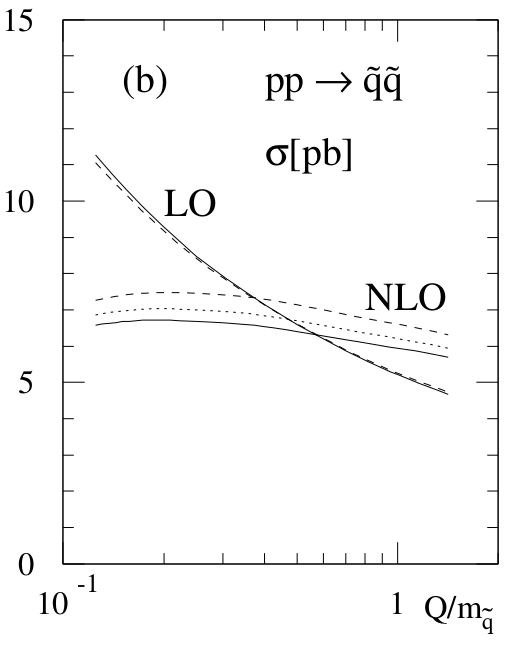
\includegraphics[scale=0.4]{squark_gluino_LO_NLO.png}
\caption{The dependence on the renormalization/factorization scale $Q$ of the LO and NLO cross sections for squark-squark production at the LHC ($\sqrt{s}=14$ TeV). Parton densities are GRV94 (solid), CTEQ3 (dashed) and MRS(A') (dotted). Mass parameters are $m_{\tilde{q}}=600$ GeV, $m_{\tilde{g}}=500$ GeV and $m_t=175$ GeV. Figure from \cite{beenakker1997squark}.}
\label{Fig:: hadron susy : LO vs NLO beenakker}
\end{figure}


The calculations from \cite{beenakker1997squark} assume degenerate squark masses $m_{\tilde{q}}$, set the 5 lightest quark masses to zero as they are much lighter than the squarks, and the top quark mass to $m_t =175$ GeV. The two free parameters left are then $m_{\tilde{g}}$ and $m_{\tilde{q}}$. This indicates that these might be good features for the learning. The renormalization scheme used is the $\bar{MS}$ scheme. Masses and couplings are renormalized, and the resulting parameters can be found in \cite{beenakker1997squark}.

\subsubsection{Partonic Cross-Section}

As previously discussed, calculations for hadron colliders require first finding the hadronic cross sections. In order to analyze these, scaling functions are introduced \cite{beenakker1997squark}
\begin{align}
\hat{\sigma}_{ij} = \frac{\alpha_s^2(Q^2)}{m^2} \Big\{ f^B_{ij}(\eta, r) + 4 \pi \alpha_s (Q^2) \Bigg[ f_{ij}^{V+S}(\eta, r, r_t) + f_{ij}^H (\eta, r) + \bar{f}_{ij} (\eta, r) \log \Bigg( \frac{Q^2}{m^2}\Bigg) \Bigg] \Big\}
,
\end{align}
where $Q^2$ is the mass scale, often set to $Q^2 = m^2$, and $m^2 = (\sqrt{p_1^2} + \sqrt{p_2^2})/2$ is the mass of the final particles. The scaling functions $f$ are as follows: the Born term $f^B$, the sum of virtual and soft-gluon corrections $f^{V+S}$, the hard gluon corrections $f^H$, and the scale-dependent contributions $\bar{f}$. The partonic cross section depends on the parameters
\begin{align}
&\eta = \frac{s}{4m^2} -1, &r= \frac{m_{\tilde{g}}^2}{m_{\tilde{q}}^2}, &&r_t = \frac{m_t^2}{m^2},
\end{align}
which may be used in deciding the target and features for the learning process.

\subsubsection{Hadronic Cross-Section}

As per the previous discussion, the partonic cross-sections must be integrated over in order to obtain the total hadronic cross section. A convolution integral over the parton distribution functions yields the expression 
\begin{align}
\sigma(S, Q^2) = \sum_{i,j=q, q, \bar{q}} \int_{\tau}^1dx_1 \int_{\tau/x_1}^1 dx_2 f_i^{h_1} (x_1, Q^2) f_j^{h_2}(x_2, Q^2) \hat{\sigma}_{ij} (x_!x_2S, Q^2)\Big|_{\tau=4m^2/S}.
\end{align}
The integrals are calculated numerically using the VEGAS integration routine \cite{PETERLEPAGE1978192} in \cite{beenakker1997squark}.
The uncertainty due to different parameterizations of the parton densities for the LHC calculations of the NLO terms amount to $\lesssim 13 \%$ at the central scale.

\subsubsection{K-Factor}

To quantify the improvement on the cross section found by adding NLO terms, the \textit{K-factor} is introduced. It is the ratio between the cross sections
\begin{align}
K = \sigma_{NLO}/\sigma_{LO}.
\end{align}
The $K$-factor for squark production for varying mass ratios $m_{\tilde{q}}/m_{\tilde{g}}=2.0, 1.6,1.2,0.8$ at the LHC is shown in Fig. (\ref{Fig:: susy hadron : K-factor LHC}). As seen from the figure, the $K$-factor is larger than 1 and quite stable as a function of the squark mass. This indicates a shift in the mass spectrum, and provides stronger bounds on particle masses.

\begin{figure}
\centering
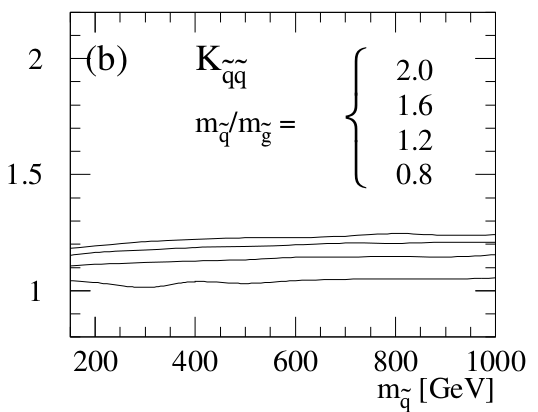
\includegraphics[scale=0.5]{squark_gluino_K_factor.png}
\caption{The $K$-factors for the LHC ($\sqrt{s}=14$ TeV). Parton densities are GRV94, with scale $Q=m$, and the top squark mass is $m_t=175$ GeV. Figure from \cite{beenakker1997squark}.}
\label{Fig:: susy hadron : K-factor LHC}
\end{figure}


\subsection{State-of-the-art Tools}

There are several numerical tools available for the calculation of NLO SUSY cross sections. Two of them are here considered, namely Prospino \cite{beenakker1996prospino} and NLL-fast \cite{beenakker2016nlo+}.

\subsubsection{Prospino}\label{sec:Prospino}
A tool that uses the $K$-factor to calculate NLO cross sections is \verb|Prospino 2.1| \cite{beenakker1996prospino}. \verb|Prospino 2.1| has the advantage of calculating cross sections with \textit{non-degenerate} squark masses. This is done by first computing LO cross sections for the 5 or 4 lightest squark flavors, saved in the $LO\_ms$ parameter. The LO and NLO rates are then calculated for a mean value of the squark mass, and the corresponding $K$-factor is calculated. These values are given as $LO$ and $NLO$. The $LO\_ms$ values are then multiplied by the $K$-factor, giving an approximation to the NLO terms for non-degenerate masses, given as $NLO\_ms$. The calculations are outlined in the section above, and are described in more detail in \cite{beenakker1996prospino}. This does mean, however, that calculations take very long. Evaluating the strong process cross sections for just a single CMSSM benchmark point takes about 15 minutes of CPU time on a modern processor \cite{balazs2017colliderbit}. In addition, as was discovered during the project, \verb|Prospino 2.1| has a weakness in the heavy squark mass space. Consider the cross section for the production of $\tilde{c}_L \tilde{c}_L$. When all squark masses are heavy, but $m_{\tilde{c}_L}$ is slightly lighter than the others, the $K$-factor is set to zero, possibly due to a numerical error. This means that $LO \neq 0$ and $NLO =0$, which gives problematic outlier points that cause trouble during learning.



\subsubsection{NLL-fast}

\verb|NLL-fast 2.1| \cite{beenakker1997squark, kulesza2009threshold, kulesza2009soft, beenakker2009soft, beenakker2011squark} computes the hadronic cross sections of gluino and squark pair production including NLO supersymmetric QCD corrections, and the resummation of soft gluon emission at next-to-leading-logarithmic (NLL) accuracy. It also provides a theoretical error estimation, based on the errors from scale dependence and the parton distribution functions. The calculation is done by reading in LO and NLO+NLL results, the scale uncertainty and the pdf and alphas error, and uses fast interpolation to calculate cross sections for any squark and gluino mass approximately within the range $[200, 1500]$ GeV. This does mean, however, that \verb|NLL-fast 2.1| only calculates cross sections for mass-degenerate squarks.

\subsubsection{Accuracy}

Including the NLO cross sections has reduced the theoretical error to be as low as $10 \%$ for a wide range of processes and masses, see the discussion in \cite{balazs2017colliderbit}. There are other uncertainties, however, such as the ones from the PDFs and $\alpha_s$. These must also be included in the total error estimate. PDFs are based on experimental data, and so the uncertainty increases with the sparticle masses because the PDFs are most poorly constrained at large scales and at large partons $x$.

To illustrate, consider both the gluino and (degenerate) squark mass to be $1.5$ TeV, which is at the edge of what the LHC is able to produce at 8 TeV. \verb|NLL-fast 2.1| then gives errors of $(+24.3 \%, -22.2\%)$ for the PDFs and $(+8.3 \%, -7.3 \%)$ for $\alpha_s$, when using the MSTW2008 NLO PDF
set \cite{Martin:2009iq}. In this case the total error will not be much lower than $25 \%$. 

Thus, the relative errors obtained in this thesis should not exceed $10 \%$, in order to improve on the existing methods.




\bibliographystyle{plain}
\bibliography{dingsen_susy_at_hadron_colliders}



\bibliographystyle{plain}
\bibliography{dingsen_gaussian_processes}




\chapter*{Appendix A: The Gaussian Distribution}


\bibliographystyle{plain}
\bibliography{dingsen}

\chapter*{Appendix B: Benchmarks}

\section{When the Error is Known}

Most observations are noisy versions of the true function values. In \cite{rasmussen2006gaussian} there is an example using additive independent identically distributed Gaussian noise $\varepsilon$ with variance $\sigma_n^2$ (and standard deviation $\sigma_n$). The benchmark function attempts to convert the noisy function at hand to the form
\begin{align}\label{Eq:: Gaussian noise}
y = f(x) + \varepsilon \text{ , } \varepsilon \sim  \mathcal{N} (0, \sigma_n).
\end{align}

This may, according to \ref{Eq:: cross section log gaussian noise}, be done. Assume a relatively simple function which spans over several orders of magnitude, with a shape that can easily be modelled by the RBF kernel. The function used here is
\begin{align}
f(x) =  1000 \exp \Big(-\frac{x^2}{10}\Big) \text{ , } x \in [0, 30],
\end{align} 
with a corresponding noisy function 
\begin{align}
y = f(x) + \varepsilon f(x),
\end{align}
where $\varepsilon \sim \mathcal{N} (0, \sigma_n^2)$.

A plot of the true function and noisy function, along with their logarithms, are shown in Fig. (\ref{Fig:: y and fx} -\ref{Fig:: log y and log fx}). A large standard deviation for the error is used for illustrational purposes. The error is relatively much smaller for the log of functions, and more evenly distributed, as can be seen from the zoom in in Fig (\ref{Fig:: log y and log fx zoom}).

\begin{figure}
\centering
\includegraphics[scale=0.3]{/home/ingrid/Documents/Master/ML/Benchmarks/known_error/y_fx_alpha01.pdf}
\caption{The pure and noisy function with $\varepsilon \sim \mathcal{N} (0, \sigma_{std} = 0.1)$.}
\label{Fig:: y and fx}
\end{figure} 

\begin{figure}
\centering
\includegraphics[scale=0.3]{/home/ingrid/Documents/Master/ML/Benchmarks/known_error/y_fx_log_alpha01.pdf}
\caption{The logarithm of the pure and noisy function with $\varepsilon \sim \mathcal{N} (0, \sigma_{std} = 0.1)$.}
\label{Fig:: log y and log fx}
\end{figure} 

\begin{figure}
\centering
\includegraphics[scale=0.3]{/home/ingrid/Documents/Master/ML/Benchmarks/known_error/y_fx_log_alpha01_zoom.pdf}
\caption{The logartihm of the pure and noisy function with $\varepsilon \sim \mathcal{N} (0, \sigma_{std} = 0.1)$.}
\label{Fig:: log y and log fx zoom}
\end{figure} 

For the actual training and prediction, a standard deviation of $\sigma_{std} = 0.001$ was used (to get a similar number to the real case of the cross sections). A single Gaussian process was performed with 500 training points and 4000 test points, using the RBF kernel. The Gaussian process was first tested on the true function, and the error measure was the relative error given by
\begin{align}
\epsilon_{GP} = \frac{y_{true} - y_{predicted}}{y_{true}},
\end{align}
where $y_{predicted} = 10^{\log_{10} f_{predicted}}$, and $f_{predicted}$ is what the GP predicts. The optimal hyperparameters for the RBF kernel on the true function were
\begin{align*}
\text{kernel}_{true} = 3.16^2 \exp \Big( - \frac{x^2}{5.6^2} \Big),
\end{align*}
with no noise. A histogram of the errors is shown in Fig. (\ref{Fig:: fx prediction no noise}).

\begin{figure}
\centering
\includegraphics[scale=0.3]{/home/ingrid/Documents/Master/error_investigation/fx_log_nowk.pdf}
\caption{Error histogram of the Gaussian process prediction for the true function $f(x)$ using a noiseless RBF-kernel.}
\label{Fig:: fx prediction no noise}
\end{figure}

The prediction for the error is
\begin{align*}
\Big( \frac{\varepsilon}{\log 10} \Big)^2 = \frac{(1 \cdot 10^{-3})^2}{(\log 10)^2} = 1.886 \cdot 10^{-7}.
\end{align*}

Setting $\alpha = 1.886 \cdot 10^{-7}$ gives the best prediction, with a kernel with very similar hyperparameters to the noise-free case
\begin{align}
\text{kernel}_{noisy} = 3.16^2 \exp \Big( - \frac{x^2}{5.82^2} \Big).
\end{align}

It also improves the prediction significantly from the case where no noise is fed to the estimator. A plot of the case where $\alpha = 10^{-10}$ and $\alpha = 1.886 \cdot 10^{-7}$ are shown in Fig. (\ref{Fig:: y prediction no noise}) and Fig. (\ref{Fig:: y prediction alpha=1.886}), respectively.

\begin{figure}
\centering
\includegraphics[scale=0.3]{/home/ingrid/Documents/Master/error_investigation/y_log_nowk.pdf}
\caption{Error histogram of the Gaussian process prediction for the noisy function $y(x)$ using a noiseless RBF-kernel ($\alpha = 10^{-10}$).}
\label{Fig:: y prediction no noise}
\end{figure}

\begin{figure}
\centering
\includegraphics[scale=0.3]{/home/ingrid/Documents/Master/error_investigation/y_log_alpha1886min7.pdf}
\caption{Error histogram of the Gaussian process prediction for the noisy function $y(x)$ using an RBF-kernel with $\alpha = 1.886 \cdot 10^{-6}$.}
\label{Fig:: y prediction alpha=1.886}
\end{figure}

The best value for $\alpha$ is in fact very close to our estimate, as can be seen from Fig. (). Note that $\alpha \propto 10^{-8}$ gives a smaller mean than $\alpha \propto 10^{-7}$, but it also has a much larger variance.

\begin{figure}
\centering
\includegraphics[scale=0.3]{/home/ingrid/Documents/Master/error_investigation/y_log_sigma_alpha.pdf}
\caption{Standard deviation of error distribution of the Gaussian process prediction for a varying noise level variance $\alpha$.}
\label{Fig:: y prediction alpha mu}
\end{figure}



\chapter{Gaussian Processes}

In this chapter Gaussian process regression is introduced. First, some concepts and expressions in Bayesian statistics are reviewed. The following section introduces the mathematical framework needed for Gaussian processes, before selected covariance functions are discussed. Concepts in Bayesian model selection are used as a basis to quantify and improve the quality of predictions. Finally, distributed Gaussian processes are introduced as a way of scaling Gaussian processes to larger datasets.

\section{Introduction to Bayesian Statistics}

There are two general philosophies in statistics, namely \textit{frequentist} and \textit{Bayesian} statistics. To understand where they differ, consider a statement statisticians from both branches consider to be true

\begin{center}
\textit{Statisticians use probability to describe uncertainty.}
\end{center}

The difference between Bayesian and frequentist statistics is at the definition of the \textit{uncertain}. Since uncertainty is described by probability this must also vary, and one distinguishes between \textit{objective} and \textit{subjective} probability. Consider an example in which a statistician throws a dice. Before throwing, he is uncertain about the outcome of the dice toss. This uncertainty related to the outcome is \textit{objective}: no one can know if he will throw a 1 or a 4. On the other hand, he might also be uncertain about the underlying probability distribution of the dice toss. Is the dice loaded? Is one of the edges sharper than the others? This uncertainty is \textit{subjective}, as it may vary depending on how much information is available about the system. One of the main critiques of subjective probability posed by frequentists is that the final probability depends on who you ask.

\subsection{Bayes' Theorem}

To further illustrate the difference between frequentist and Bayesian statistics \textit{Bayes' theorem} is introduced. Bayes' theorem can be derived from the familiar rules of probability
\begin{align}\label{Eq:: Sum rule}
P(X | I) + P(\bar{X} | I) = 1,
\end{align}
\begin{align}\label{Eq:: Product rule}
P(X, Y | I) = P(X | Y, I) \times P(Y | I),
\end{align} 
commonly known as the \textit{sum rule} and \textit{product rule}, respectively. $P(X|I)$ is the probability of outcome $X$ given the information $I$, and $P(X|Y,I)$ is the probability of outcome $X$ given the information $I$ \textit{and} outcome $Y$. The bar over $\bar{X}$ means that the outcome $X$ does \textit{not} happen. The sum rule states that the total probability of the outcomes $X$ and $\bar{X}$ is equal to 1. This is rather untuitive, considering an event either takes place not. The second rule, the product rule, states that the probability of both outcomes $X$ and $Y$ is equal to the probability of $Y$ times the probability of $X$ given that $Y$ has ocurred. These expressions combine to give Bayes' theorem, first formulated by reverend Thomas Bayes in 1763,
\begin{align}\label{Eq:: gaussian process : Bayes theorem}
P(X | Y, I) = \frac{P(Y | X, I) \times P(X | I)}{P(Y | I)}.
\end{align}
This theorem states that the probability of $X$ given $Y$ equals the probability of $Y$ given $X$ times the probability of $X$, divided by the probability of $Y$. Surprisingly, there is nothing Bayesian about Bayes' theorem. It merely reformulates the rules of logical consistent reasoning stated by Richard Cox in 1946 \cite{sivia2006data}. Laplace was the one to make Bayes' theorem Bayesian, when he used the theorem to perform inference about distribution parameters. These are, for example, the mean and variance of a Gaussian distribution. The resulting expression is
\begin{align}
P(\Theta = \theta | X=x) = \frac{P(X=x|\Theta = \theta) P(\Theta = \theta)}{P(X=x)},\label{Eq:: gaussian process : Bayesian inference}
\end{align}
where $\Theta$ are the possible probability distribution parameters, $X$ are the possible outcomes, $P(X=x)$ is a normalization constant called the \textit{marginal likelihood}, and $P(X=x|\Theta = \theta)$  and $P(\Theta = \theta)$ are the \textit{likelihood} and \textit{prior}, respectively. In other words, Eq.\ (\ref{Eq:: gaussian process : Bayesian inference}) states the probability of the parameters $\theta$ given the knowledge of outcomes $x$.

A crucial parting of Bayesian statistics from frequentist statistics is at the introduction of the \textit{prior}, which expresses a probability distribution on the \textit{parameters} of the probability distribution.

\subsection{Priors and Likelihood}

The likelihood $P(X = x |\Theta = \theta)$ is simply the probability of the observations $x$ given the parameters of the probability distribution $\theta$. Conversely, the prior expresses a prior belief or assumption of the data, and has to be determined beforehand. The measure $P(\Theta = \theta | X = x)$ from Eq. (\ref{Eq:: gaussian process : Bayesian inference}) is called the \textit{posterior distribution}. This can be thought of as the prior belief, modified by how well this belief fits the data,
\begin{align*}
\text{posterior} = \frac{\text{prior} \times \text{likelihood}}{\text{marginal likelihood}}.
\end{align*}
Consider an example. The statistician from before now sets about tossing a coin. Before tossing he assumes the probability of all outcomes is equal, and so adopts a flat prior probability distribution. After one throw he gets heads, and the posterior changes to a function with high probability for heads, and low for tails. After 4 throws where two were heads and two were tails the posterior shows an equal probabilty for heads and tails, with a wide distribution centered at 0.5. After several throws the distribution converges to a narrow peak around $0.25$, illustrated in Fig.\ (\ref{Fig:: gaussian process : Dice throw }). This indicates an unfair coin that is biased towards tails.

\begin{figure}
\includegraphics[scale=0.85]{figures_gaussian_processes/coin_toss_xd.pdf}
\caption{The posterior probability distribution of the bias-weighting of a coin for the uniform prior, $P(H|I)$. The first panel from the left is before the coin is tossed, the second panel is after 1 toss, the third is after 4 tosses, and the fourth is after 1024 tosses. The posterior converges towards a narrow peak at $0.25$, so the coin is biased.}
\label{Fig:: gaussian process : Dice throw }
\end{figure}


\subsection{Best Estimate and Reliability}

Given a posterior distribution it is important to decide how well it fits the data. For that purpose the \textit{best estimate} and \textit{reliability} are defined. The best estimate $X_0$  is the outcome with the highest probability. In other words, it is the maximum of the posterior
\begin{align}
&\frac{dP}{dX}\Big|_{X_0} = 0, &\frac{d^2P}{dX^2}\Big|_{X_0} < 0.
\end{align}
The second derivative must be negative to insure that $X_0$ is, in fact, a maximum. Equally important to finding a best estimate is knowing how reliable the estimate is. Reliability is connected the width of the distribution, or how much the data is smeared out. A narrow distribution has low uncertainty, while a wide distribution has large uncertainty. The width is found by Taylor expanding the posterior, and taking the logarithm \footnote{$L$ is a monotonic function of $P$, so the maximum of $L$ is at the maximum of $P$.}
\begin{align}
&L = L(X_0) + \frac{1}{2} \frac{d^2}{dx^2} L\Big|_{X_0} (X-X_0)^2 +... ,&L = \log_e \Big[\text{prob}(x | \{data\}, I) \Big]\label{Eq:: gaussian process : Taylor expansion L}
\end{align}
This gives an approximate posterior in the shape of a \textit{Gaussian distribution}, with mean and variance given by
\begin{align}
&\mathcal{N}( \mu, \sigma) \text{ where } \mu = X_0\text{, } \sigma = \Big( - \frac{d^2L}{dx^2} \Big)^{-1/2}.
\end{align}
The Gaussian distribution is symmetric with respect to the maximum at $x = \mu$, and has a full width at half maximum (FWHM) at around $2.35 \sigma$, as shown in Fig. (\ref{Fig:: gaussian process : Gaussian distribution}).

\begin{figure}
\centering
\includegraphics[scale=1.5]{figures_gaussian_processes/gaussian_distribution_xd.pdf}
\caption{A Gaussian probability distribution. The maximum is at the mean value $\mu$, with a full width at half maximum (FWHM) at around $2.35 \sigma$. Figure from \cite{sivia2006data}.}
\label{Fig:: gaussian process : Gaussian distribution}
\end{figure}

\subsection{Covariance}

Before embarking on Gaussian processes the concept of \textit{covariance} is needed. A more detailed description is found in \cite{sivia2006data}. In many cases the equations are not as simple to solve as in Eq.\ (\ref{Eq:: gaussian process : Taylor expansion L}), as the probability distribution might have several quantities of interest $\{ X_i \}$. In that case, a set of \textit{simultaneous equations} must be solved to get the best estimate
\begin{align}\label{Eq:: gaussian process : Best estimate X_i}
\frac{dP}{dX_i} \Big|_{X_{0j}} =0.
\end{align}
To simplify expressions consider the problem in two dimensions, so that $\{ X_i \} = (X, Y)$. The Taylor expansion of $L$ is then
\begin{align}\label{Eq:: gaussian process : Taylor expansion L_i}
L =& L(X_0, Y_0) + \frac{1}{2} \Big[ \frac{d^2L}{dX^2}  \Big|_{X_0, Y_0}(X-X_0)^2 \nonumber \\
& + \frac{d^2L}{dY^2}  \Big|_{X_0, Y_0}(Y-Y_0)^2 + 2 \frac{d^2L}{dXdY}  \Big|_{X_0, Y_0}(X-X_0)(Y-Y_0) \Big] +...
\end{align}
There are now four partial derivatives, reduced to three using the rules for mixed partial derivatives $\frac{\partial^2}{\partial X \partial Y} = \frac{\partial^2}{\partial Y \partial X}$. Writing the quadratic term of Eq.~\ref{Eq:: gaussian process : Taylor expansion L_i} in matrix form gives
\begin{align}
Q = 
\begin{pmatrix}
X-X_0 & Y -Y_0
\end{pmatrix}
\begin{pmatrix}
A & C\\
C & B
\end{pmatrix}
\begin{pmatrix}
X -X_0\\
Y-Y_0
\end{pmatrix},
\end{align}
where the matrix elements are
\begin{align}
&A = \frac{\partial^2 L}{\partial X^2} \Big|_{X_0, Y_0}, &B = \frac{\partial^2 L}{\partial Y^2} \Big|_{X_0, Y_0}, &&C = \frac{\partial^2 L}{\partial X \partial Y} \Big|_{X_0, Y_0}.
\end{align}
The \textit{variance} is defined as the expectation value of the square of deviations from the mean. In the two-dimensional case this becomes \cite{sivia2006data}
\begin{align}
\text{Var}(X) = \sigma_x^2 = \braket{(X - X_0)^2} = \int \int (X - X_0)^2 P (X, Y | \{\text{data}\}, I) dXdY.
\end{align}
This is the variance $\sigma_X^2$ for $X$, and its square root is the standard deviation $\sigma_X$. A similar expression can be found for $Y$, by switching $X$ and $Y$. It is also possible to find the simultaneous deviations of the parameters $X$ and $Y$, or the correlation between the inferred parameters. This is called the \textit{covariance} $\sigma_{XY}^2$, and is in two dimensions given by
\begin{align}
\sigma_{XY}^2 = \braket{(X - X_0) (Y - Y_0)} =\int \int (X - X_0) (Y - Y_0) P (X, Y | \{\text{data}\}, I) dXdY.
\end{align}
The covariance indicates how an over- or underestimation of one parameter affects another parameter. If, for example, an overestimation of $X$ leads to an overestimation of $Y$, the covariance is positive. If the overestimation of $X$ has little or no effect on the estimation of $Y$, the covariance is negligible or zero $|\sigma_{XY}| \ll \sqrt{\sigma_X^2 \sigma_Y^2}$. These effects are illustrated in Fig.\ (\ref{Fig:: gaussian process : Covariance illustrated}). It can be shown that \cite{sivia2006data}
\begin{align}
\text{cov} = 
\begin{pmatrix}
\sigma_X^2 & \sigma_{XY}^2\\
\sigma_{XY}^2 & \sigma_Y^2
\end{pmatrix}
= - \begin{pmatrix}
A & C\\
C & B
\end{pmatrix}^{-1}.
\end{align}
This is called the \textit{covariance matrix}.

\begin{figure}
\centering
\includegraphics[scale=1.0]{figures_gaussian_processes/covariance_xd.pdf}
\caption{A schematic illustration of covariance and correlation. (a) The contours of a posterior pdf with zero covariance, where the inferred values of $X$ and $Y$ are uncorrelated. (b) The corresponding plot when the covariance is large and negative; $Y + mX =$ constant along the dotted line (where $m > 0$), emphasizing that only this sum of the two parameters can be inferred reliably. (c) The case of positive correlation, where we learn most about the difference $Y − mX$; this is constant along the dotted line.}
\label{Fig:: gaussian process : Covariance illustrated}
\end{figure}


\section{Gaussian Process Regression}

Gaussian processes (GP) is a supervised machine learning method, designed to solve regression and probabilistic classification problems. In this thesis only regression will be used. 

%As experience dictates that Gaussian processes can be hard to grasp, it will serve both the reader and the author well to begin on a conceptual level: \textit{what do Gaussian processes do?}

Consider a set of points $\mathcal{D} = \{\textbf{x}_i, y_i\}$, where $y$ is some (possibly noisy) function of $\textbf{x}$, $y = f(\textbf{x}) + \varepsilon$. This is illustrated by the black dots in in Fig. (\ref{Fig:: gaussian process : GP illustration}). In machine learning $\mathcal{D}$ is the \textit{training data}, as it is used to train the model. It consists of \textit{features}, which are the input vectors $\textbf{x}_i$, and \textit{targets}, which are the function values $y_i$. The set of points is discrete, so there is some $\textbf{x}^*$ for which the target $y^*$ is unknown. Gaussian Processes (GP) predict a Gaussian distribution \textit{over function values} at this point $\textbf{x}^*$, with a corresponding mean $m(\textbf{x}^*)$ and variance $\sigma^2$. The GP prediction for the target value $y^*$ is the mean $m(\textbf{x}^*)$, with uncertainty $\sigma^2$. The predicted target $y^*$ can be viewed as a linear combination of the known targets $y_i$, where the weights are controlled by the covariances between $\textbf{x}_i$ and the test point $\textbf{x}^*$.  


\begin{figure}
\centering
\includegraphics[scale=1.5]{figures_gaussian_processes/gp_illustration_xd.pdf}
\caption{An illustration of a GP prediction of the target value $y^*$ (blue cross), given the known set of points $\{x_i, y_i\}$ (black dots). The prediction is a Gaussian distribution in $y$ with mean $y^*$ and variance $\sigma^2$. The Gaussian distribution is drawn in red with $y$ on the vertical axis, with uncertainty in the $y$-direction.}
\label{Fig:: gaussian process : GP illustration}
\end{figure}

\subsubsection{Function Space View}

Since Gaussian processes provide distributions over functions, it is useful to consider the problem in the function space view introduced in \cite{rasmussen2006gaussian}. For a real process $f(\textbf{x})$ the mean  $m(\textbf{x})$ and covariance function $k(\textbf{x}, \textbf{x}')$ are defined as
\begin{align}
m(\textbf{x}) &= \mathbb{E}[f(\textbf{x})],\\
k(\textbf{x}, \textbf{x}') &= \mathbb{E} [(f(\textbf{x}) - m(\textbf{x}))(f(\textbf{x}') - m(\textbf{x}'))],
\end{align}
where $\mathbb{E}[a]$ is the expectation value of some quantity $a$. Given the mean and covariance, the Gaussian distribution for $f(\textbf{x})$ is completely specified
\begin{align}
f(\textbf{x}) \sim \mathcal{GP}(m(\textbf{x}), k(\textbf{x}, \textbf{x}')).
\end{align}
The covariance between two points $k(\textbf{x}_i, \textbf{x}_j)$ is decided by the \textit{kernel function}. In this text the running example will be the squared exponential (SE) kernel, given by
\begin{align}
k(f(\textbf{x}_i), f(\textbf{x}_j)) = k(\textbf{x}_i, \textbf{x}_j) = \exp \Big( - \frac{1}{2} |\textbf{x}_i - \textbf{x}_j|^2 \Big).
\end{align}
Note that the covariance of the function values $f(\textbf{x}_i)$, $f(\textbf{x}_j)$ only depends on the input parameters $\textbf{x}_i$, $\textbf{x}_j$. 

Specifying the covariance function specifies a distribution over functions \cite{rasmussen2006gaussian}. This is because allowed functions must obey the correlation decided by $k(\textbf{x}_i, \textbf{x}_j)$. Using the kernel on a set of input vectors contained in the matrix $X^*$, gives the \textit{covariance matrix}. Combined with an initial mean of zero \footnote{The mean does not have to be zero, it could for example be the mean of the training data.} one obtains the \textit{prior} distribution
\begin{align}
f(x) \sim \mathcal{N} (0, K(X^*, X^*)).
\end{align} 
This distribution encodes the prior knowledge about the function values $f(x)$, and so the choice of kernel is one of the most important steps in learning with GPs. The prior is modified by the training data to provide a posterior distribution. In Fig.\ (\ref{Fig:: gaussian process : prior posterior drawn samples}) samples are drawn from both the prior and posterior distribution. Samples are here taken to mean functions that obey the covariance function. In the case of the prior, the samples are drawn from a distribution of functions with mean zero and constant variance, meaning that if you drew enough functions the mean value of all functions at every $x$ would be zero. For the posterior, the mean values and uncertainties have been modified by the training data. In a point where there is training data the uncertainty is zero \footnote{Assuming there is no noise in the data.}, and so all samples drawn from this distribution must pass through this point. Far away from training points the uncertainty is large.

\begin{figure}
\centering
\includegraphics[scale=0.55]{figures_gaussian_processes/draw_samples_benchmark.pdf}
\caption{Drawing functions from the prior (top) and posterior (bottom) distributions. The thick, black line represents the mean of the distribution, while the shaded, blue area is the uncertainty. The multiple colored lines are functions drawn randomly from the prior and posterior distributions, whose correlation are dictated by the covariance function. The prior has mean 0 and covariance given by the squared exponential function. The posterior has been modified by training points (red dots), giving rise to zero uncertainty at the points where training data exists, and an altered mean value for the distribution. Figure generated using scikit-learn.}
\label{Fig:: gaussian process : prior posterior drawn samples}
\end{figure}

Consider a simple example of a noise-free set of training points $\{\textbf{x}_i, y_i\}$, so that $y = f(\textbf{x})$. The joint distribution of training outputs $\textbf{f}$ and test outputs $\textbf{f}^*$ according to the prior is then
\begin{align}
\begin{bmatrix}
\textbf{f}\\
\textbf{f}^*
\end{bmatrix}
\sim 
\mathcal{N} \Bigg(
\boldsymbol{0},
\begin{bmatrix}
K(X, X) & K(X, X^*)\\
K(X, X^*) & K(X^*, X^*)
\end{bmatrix}
 \Bigg)
\end{align}
For $n$ training points and $n^*$ test points, $K(X,X)$ is the $n \times n$ matrix containing the covariance of training points, $K(X, X^*)$ is the $n \times n^*$ matrix of covariance between the test and training points, and $K(X^*, X^*)$ is the $n^* \times n^*$ matrix containing the covariance of test points. By conditioning the distribution of $\textbf{f}^*$ on the observations,  the posterior distribution over $\textbf{f}^*$ is obtained\footnote{For more details, see Appendix A.2 in \cite{rasmussen2006gaussian}.}  \cite{rasmussen2006gaussian} 
\begin{align}
\textbf{f}_* \big| X_*, X, \textbf{f} \sim \mathcal{N}&(K(X_*, X)K(X, X)^{-1} \textbf{f},\\ &K(X_*, X_*) - K(X_*, X)K(X, X)^{-1}K(X, X_*)).
\end{align}

\subsubsection{Gaussian Noise Model}

Noise-free observations are rare. In most cases targets will contain some noise $y = f(\textbf{x}) + \varepsilon$, where the noise $\varepsilon$ is assumed to follow a Gaussian distribution $\varepsilon \sim \mathcal{N}(0, \sigma_n^2)$. This is the \textit{Gaussian noise model}. The covariance can then be expressed as
\begin{align}
&\text{cov}(y_i, y_j) = k(\textbf{x}_i, \textbf{x}_j) + \sigma_n^2 \delta_{ij} 
\end{align}
which gives for the prior distribution
\begin{align}
\begin{bmatrix}
\textbf{y}\\
\textbf{f}^*
\end{bmatrix}
\sim 
\mathcal{N} \Bigg(
\boldsymbol{0},
\begin{bmatrix}
K(X, X) + \sigma_n^2 \mathbb{I} & K(X, X^*)\\
K(X, X^*) & K(X^*, X^*)
\end{bmatrix}
 \Bigg).
\end{align}
The conditioned distribution is then 
\begin{align}
\textbf{f}^* \big| X^*, X, \textbf{f} & \sim \mathcal{N}(\bar{\textbf{f}}^*, \text{cov}(\textbf{f}^*)), \text{ where} \\
\bar{\textbf{f}}^* &= K(X^*, X) [K(X, X) + \sigma_n^2 \mathbb{I}]^{-1} \textbf{y},\\
\text{cov} (\textbf{f}^*) &= K(X^*, X^*) - K(X^*, X)[K(X, X) + \sigma_n^2 \mathbb{I}]^{-1} K(X, X^*) 
\end{align}

For the sake of tidying up the expression define the matrix $K \equiv K(X, X)$ and the matrix $K^* \equiv K(X, X^*)$. In the case of a single test point $\textbf{x}^*$ the matrix $K^*$ is written as a vector $\textbf{k}(\textbf{x}^*) = \textbf{k}^*$. Using this compact notation the GP prediction for a single test point $\textbf{x}^*$ is
\begin{align}
\bar{f}^* &= \textbf{k}^{*T}(K + \sigma_n^2\mathbb{I})^{-1} \textbf{y},\label{Eq:: gaussian process : GP prediction mean}\\
\mathbb{V}[f^*] &= k(\textbf{x}^*, \textbf{x}^*) - \textbf{k}^{*T}(K + \sigma_n^2 \mathbb{I})^{-1} \textbf{k}^*\label{Eq:: gaussian process : GP prediction variance}.
\end{align}
Note that the predicted mean value $\bar{f}^*$ can be viewed as a linear combination of $y_i$ of the form $\alpha \textbf{y}$, where $\alpha = \textbf{k}^{*T}(K + \sigma_n^2\mathbb{I})^{-1}$. $\alpha$ then only contains the covariance between features.

Eqs. (\ref{Eq:: gaussian process : GP prediction mean})-(\ref{Eq:: gaussian process : GP prediction variance}) form the basis for GP prediction in \verb|scikit-learn|  \cite{scikit-learn}. The algorithm is shown in Algorithm (\ref{Alg:: gaussian process : GP}), and uses the Cholesky decomposition of the covariance matrix.

\begin{algorithm}
\KwData{$X$ (inputs), \textbf{y} (targets), $k$ (covariance function/kernel), $\sigma_n^2$ (noise level), $\textbf{x}_*$ (test input).}
L = Cholesky decomposition ($K + \sigma_n^2 I$) \;
$\boldsymbol{\alpha} = (L^T)^{-1}(L^{-1} \textbf{y})$ \;
$\bar{f}_* = \textbf{k}_*^T \boldsymbol{\alpha}$ \;
$\textbf{v} = L^{-1} \textbf{k}_*$ \;
$\mathbb{V}[f_*] = k(\textbf{x}_*, \textbf{x}_*) - \textbf{v}^T \textbf{v}$ \;
$\log p(\textbf{y}|X) = - \frac{1}{2} \textbf{y}^T \boldsymbol{\alpha} - \sum_i \log L_{ii} - \frac{n}{2} \log 2 \pi$ \;
\KwResult{$f_*$ (mean), $\mathbb{V}[f_*]$ (variance), $\log p(\textbf{y}|X)$ (log marginal likelihood).}
\caption{Algorithm 2.1 from \cite{rasmussen2006gaussian}.}
\label{Alg:: gaussian process : GP}
\end{algorithm}

\section{Covariance Functions}
Covariance functions and kernels have been touched upon, but will be investigated further as they are central to Gaussian processes. A function that only depends on the difference between two points, $\textbf{x} - \textbf{x}'$, is called \textit{stationary}. This implies that the function is invariant to translations in input space. If, in addition, it only depends on the length $r=|\textbf{x}-\textbf{x}'|$, the function is \textit{isotropic} \footnote{Invariant to rigid rotations in input space.}.  Isotropic functions are commonly referred to as \textit{radial basis functions} (RBFs). The covariance function can also depend on the dot product, $\textbf{x} \cdot \textbf{x}'$, and is then called a \textit{dot product} covariance function.

A function which maps two arguments $\textbf{x} \in \mathcal{X}$, $\textbf{x}' \in \mathcal{X}$ into $\mathbb{R}$ is generally called a \textit{kernel} $k$. Covariance functions are symmetric kernels, meaning that $k(\textbf{x}, \textbf{x}') = k(\textbf{x}', \textbf{x})$. As previously mentioned, the matrix containing all the covariance elements is called the \textit{covariance matrix}, or the Gram matrix $K$, whose elements are given by
\begin{align}\label{Eq:: covariance matrix}
K_{ij} = k(\textbf{x}_i, \textbf{x}_j).
\end{align}

The kernel should contain information about the noise in the data, represented by a constant term added to the diagonal
\begin{align}
k(\textbf{x}_i, \textbf{x}_j)_{noise} = C \delta_{ij},
\end{align}
where $C \in \mathbb{R}$ is a real, constant number, and $\delta_{ij}$ is the Dirac delta function. In \verb|scikit-learn| this can be implemented either by giving a fixed noise level $\alpha$ to the regressor function, or by using the \verb|WhiteKernel|, which estimates the noise level from the data. This kernel is implemented in \verb|scikit-learn| in the following way for noise level $0.001$ with bounds $[10^{-10}, 1]$
\begin{lstlisting}
from sklearn.gaussian_processes.kernels import WhiteKernel
whitenoise = WhiteKernel(noise_level=0.001, noise_level_bounds=(1e-10,1))
\end{lstlisting}

\subsection{The Squared Exponential Covariance Function}

The \textit{squared exponential covariance function} (SE) has the form 
\begin{align}
k_{SE} (r) = \exp \Big( - \frac{r^2}{2 \ell^2} \Big),
\end{align} 
where $\ell$ is the \textit{characteristic length scale}. The length scale determines the smoothness of the function. For a large length scale one should expect a very slowly varying function, while a shorter length scale means a more rapidly varying function, see the illustration in Fig.\ (\ref{Fig:: gaussian process : ell variation example}). The SE  is infinitely differentiable and therefore very smooth. 

\begin{figure}
\centering
\includegraphics[scale=1.5]{figures_gaussian_processes/length_scales_xd.pdf}
\caption{The effect of varying the length scale $\ell$. A long length scale (blue) gives a smooth, slowly varying function, while a short length scale (red) gives a more staccato, quickly varying function.}
\label{Fig:: gaussian process : ell variation example}
\end{figure}

The SE is implemented in \verb|scikit-learn| under the name radial basis function, and may be called in the following way for length scale $10$, with bounds on the length scale $[0.01, 100]$
\begin{lstlisting}
from sklearn.gaussian_process.kernels import RBF
rbf = RBF(length_scale=10, length_scale_bounds=(1e-2, 1e2))
\end{lstlisting}



\subsection{The Mat\'{e}rn Class }

The \textit{Mat\'{e}rn class of covariance functions} is given by
\begin{align}
k_{Mat\acute{e}rn} (r) = \frac{2^{1- \nu}}{\Gamma (\nu)} \Big( \frac{\sqrt{2 \nu} r	}{\ell} \Big)^{\nu} K_{\nu} \Big( \frac{\sqrt{2 \nu}r}{\ell} \Big),
\end{align}
where $\nu, \ell > 0$, and $K_{\nu}$ is a modified Bessel function. The hyperparameter $\nu$ controls the smoothness of the function, as opposed to the SE kernel which is by definition very smooth. For $\nu \rightarrow \infty$ this becomes the SE kernel. In the case of $\nu$ being half integer, $\nu = p + \frac{1}{2}$, the covariance function is simply the product of an exponential and a polynomial
\begin{align}
k_{\nu=p+\frac{1}{2}} = \exp \Big(- \frac{\sqrt{2 \nu} r	}{\ell} \Big) \frac{\Gamma(p+1)}{\Gamma(2p + 1)} \sum^p_{i=0} \frac{(p+i)!}{i!(p-i)!} \Big( \frac{\sqrt{8 \nu} r	}{\ell} \Big)^{p-i}.
\end{align}
In machine learning the two most common cases are for $\nu = 3/2$ and $\nu = 5/2$
\begin{align}
k_{\nu = 3/2}(r) &=  \Big(1 + \frac{\sqrt{3}r}{\ell} \Big) \exp \Big( -\frac{\sqrt{3}r}{\ell} \Big),\\
k_{\nu = 5/2}(r) &=  \Big(1 + \frac{\sqrt{5}r}{\ell}  + \frac{5r^2}{3 \ell^2}\Big) \exp \Big( -\frac{\sqrt{5}r}{\ell} \Big).
\end{align}

In \verb|scikit-learn| the hyperparameter $\nu$ is fixed, and so not optimized during training. The Mat\'{e}rn kernel is considered more appropriate for physical processes \cite{rasmussen2006gaussian}, and may be called in \verb|scikit-learn| in the following way for length scale 10, length scale bounds $[0.01, 100]$ and $\nu = 3/2$
\begin{lstlisting}
from sklearn.gaussian_process.kernels import Matern
matern = Matern(length_scale=10, length_scale_bounds=(1e-2, 1e2), nu=1.5)
\end{lstlisting}
For values not in $\nu = [0.5, 1.5, 2.5, \infty]$ \verb|scikit-learn| evaluates Bessel functions explicitly, which increases the computational cost by a factor as high as 10.

\subsubsection{Other Kernels}

There are several kernels which are not discussed here. Kernels can be multiplied and summed to form new kernels, making the space of possible kernels infinite. For further details see chapter 4 in \cite{rasmussen2006gaussian}.





\subsubsection{Hyperparameters}

Each kernel has a vector of hyperparameters, \textit{e.g.} $\boldsymbol{\theta} = (\{M\}, \sigma^2_f, \sigma_n^2)$ for the radial basis function (RBF)
\begin{align}
k(\textbf{x}_i, \textbf{x}_j) = \sigma_f^2 \exp (- \frac{1}{2} (\textbf{x}_i - \textbf{x}_j))^T M (\textbf{x}_i - \textbf{x}_j) + \sigma_n^2 \delta_{ij}.
\end{align}
The matrix $M$ can have several forms, amongst them
\begin{align}
&M_1 = \ell^{-2} \mathbb{I} , &M_2 = \text{diag}(\vec{\ell})^{-2}.
\end{align}
Choosing $\vec{\ell}$ to be a vector in stead of a scalar is in many cases useful, especially if the vector of features contain values of different scales, \textit{e.g.} $\textbf{x} = (x_1, x_2)$ where $x_1 \in [0, 1]$ and $x_2 \in [200, 3000]$. The length scale can be set to a vector in \verb|scikit-learn| by giving the \verb|length_scale| parameter as a \verb|numpy| array of the same dimension as the feature vector $\textbf{x}$.



\section{Model Selection}

The choice of kernel and hyperparameters is important for the quality of the GP prediction. Model selection means finding the  kernel and corresponding hyperparameters that best fit the data. This is referred to as \textit{training} in machine learning. In this section Bayesian model selection is quickly overviewed, and the log marginal likelihood and cross validation are considered.

\subsection{Bayesian Model Selection}

A model has a set of model structures $\mathcal{H}_i$, hyperparameters $\boldsymbol{\theta}$ and parameters $\textbf{w}$. Feature selection is done at all levels in a hierarchical way, by finding the  posterior over \textit{parameters}, the posterior over \textit{hyperparameters} and the posterior for the \textit{model}. Here only the posterior over parameters is considered \cite{rasmussen2006gaussian},
\begin{align}
p(\textbf{w}| \textbf{y}, X, \boldsymbol{\theta}, \mathcal{H}_i) = \frac{p(\textbf{y} | X, \textbf{w}, \mathcal{H}_i) p(\textbf{w}|\boldsymbol{\theta}, \mathcal{H}_i)}{p(\textbf{y}|X, \boldsymbol{\theta}, \mathcal{H}_i)},
\end{align}
as it gives rise to the \textit{marginal likelihood} $p(\textbf{y}|X, \boldsymbol{\theta}, \mathcal{H}_i)$, given by 
\begin{align}
&p(\textbf{y}|X, \boldsymbol{\theta}, \mathcal{H}_i) = \int p(\textbf{y} | X, \textbf{w}, \mathcal{H}_i)p(\textbf{w}| \boldsymbol{\theta}, \mathcal{H}_i) d \textbf{w} & \text{(marginal likelihood)}.
\end{align}
Because of the complexity of integrals involved in model selection, it is common to maximize the marginal likelihood with respect to hyperparameters $\vec{\theta}$. This maximization is what distinguishes Bayesian model selection from other model selection schemes, as it incorporates a trade-off between model complexity and model fit. This means that a complex model will allow for several different kinds of models, but each of them will get a low probability. Meanwhile, simple models will only have a few possibilities, but each of these will have a large probability, see Fig.\ (\ref{Fig:: gaussian process : Marginal likelihood Rasmussen}).

\begin{figure}
\centering
\includegraphics[scale=1.5]{figures_gaussian_processes/marginal_likelihood_xd.pdf}
\caption{The marginal likelihood is the probability of the data, given the model. The number of data points $n$ and inputs $X$ are fixed. The horizontal axis represents an idealized set of all possible vectors of targets $\textbf{y}$. Since the marginal likelihood is a probability distribution it must normalize to unity. For a particular set $\textbf{y}'$, indicated by the dashed line, the intermediate model is preferred to the simple and complex ones.}
\label{Fig:: gaussian process : Marginal likelihood Rasmussen}
\end{figure}

%\begin{align}
%p( \boldsymbol{\theta}| \textbf{y}, X, \mathcal{H}_i) = \frac{p(\textbf{y} | X, \boldsymbol{\theta}, \mathcal{H}_i) p(\boldsymbol{\theta}| \mathcal{H}_i)}{p(\textbf{y}|X,  \mathcal{H}_i)}
%\end{align}
%\begin{align}
%p(\mathcal{H}_i| \textbf{y}, X) = \frac{p(\textbf{y} | X, \mathcal{H}_i) p( \mathcal{H}_i)}{p(\textbf{y}|X)}
%\end{align}

\subsection{Log Marginal Likelihood}

Gaussian process regression models with Gaussian noise have the wonderful trait of analytically tractable integrals for the marginal likelihood. The exact expression for the log marginal likelihood \footnote{The logarithm is used as the marginal likelihood varies rapidly.} can be shown to be \cite{rasmussen2006gaussian}
\begin{align}
\log p(\textbf{y}|X, \boldsymbol{\theta}) = - \frac{1}{2} \textbf{y}^T K_y^{-1} \textbf{y} - \frac{1}{2} \log |K_y| - \frac{n}{2} \log 2 \pi.
\end{align}
Each of the terms has an interpretation: $- \frac{1}{2} \textbf{y}^T K_y^{-1} \textbf{y}$ is the only term involving the data, and is therefore the data-fit; $-\frac{1}{2} \log |K_y|$ is the complexity penalty depending only on the covariance function and the inputs; and $- \frac{n}{2} \log 2 \pi$ is a normalization term. The marginal likelihood is conditioned on the hyperparameters of the covariance function $\vec{\theta}$, and the optimal parameters are found by maximizing. This requires the partial derivatives of the log marginal likelihood (LML)
\begin{align}
\frac{\partial}{\partial \theta_j}
 \log p(\textbf{y}|X, \boldsymbol{\theta}) = \frac{1}{2} \textbf{y}^T K^{-1} \frac{\partial K}{\partial \theta_j} K^{-1} \textbf{y} - \frac{1}{2} \text{tr} (K^{-1} \frac{\partial K}{\partial \theta_j}).
\end{align}
Computing the inverse of a matrix, $K^{-1}$, is computationally complex, and for $n$ training points goes as $\mathcal{O}(n^3)$. Once this is done, however, finding the partial derivatives only requires complexity $\mathcal{O}(n^2)$, and so gradient based optimizers are advantageous.

The LML can have several local optima, as seen in Fig. (\ref{Fig:: gaussian process : LML several local optima}). These correspond to different interpretations of the data. The rightmost optima in Fig. (\ref{Fig:: gaussian process : LML several local optima}) for example, favors a small length scale and smaller noise level. This means that it considers little of the data to be noise. The rightmost optimum has a higher noise level, and allows for several large length scales, as it considers most of the data to be noise. Features with very large length scales are considered superfluous, as the function value depends little on them. Because of this type of complication, it might be wise to restart the optimizer a few times during learning.

\begin{figure}
\centering
\includegraphics[scale=0.6]{figures_gaussian_processes/LML_two_local_maxima.pdf}
\caption{A contour plot of the log marginal likelihood with two local optima. The rightmost optima favours a short length scale and low noise, while the leftmost favors a high noise level and therefore several large length scales. Plot generated using scikit-learn.}
\label{Fig:: gaussian process : LML several local optima}
\end{figure}


\subsection{Cross Validation}

%The error of an estimator can be divided into bias, variance and noise. The bias of an estimator is the average error for differing training sets, the variance is a measure of how sensitive the estimator is to varying data, and noise is a property of the data. High bias corresponds to a model that is too simple, i.e. that it considers much of the signal to be noise, while low bias corresponds to a model that is too complicated, i.e. that it fits the data perfectly but does not model the underlying function very well. 

Cross validation is a means of monitoring the performance of a model. In k-fold validation this is done by dividing the data into $k$ subsets and using $k-1$ folds to train the model, and a single fold to validate it. This is repeated $k$ times. Cross-validation requires a loss function, such as the mean relative deviance or the $R^2$ score. The latter is given by 
\begin{align}
R^2 = 1 - \frac{\sum_{i=0}^{N-1} (y_i - \hat{y}_i)^2}{\sum_{i=0}^{N-1} (y_i - \bar{y})^2},
\end{align}
where $\hat{y}_i$ is the predicted value of the $i$th sample, $y_i$ is the true value and $\bar{y} = \frac{1}{N} \sum_{i = 0}^{N-1} y_i$ for $N$ samples. This is the score used for cross validation in this thesis.

Cross-validation can be used to plot learning curves, which is a tool to find out whether the model benefits from adding more data. The learning curve plots the training score and validation score used to find out if the model is \textit{overfitting} or \textit{underfitting}. \textit{Overfitting} means that the model is a perfect fit to the training data, but predicts poorly for test data because it is not general. \textit{Underfitting} occurs when the model is not able to capture the underlying structure of the data. 

Examples of learning curves are shown in Fig.\ (\ref{Fig:: gaussian process : learning curves}) for Naive Bayes and SVM estimators \footnote{Methods in Machine Learning.}. In a) both the training score and cross-validation score tend to a value below 1, which indicates underfitting. This model will not benefit from more data. The example in b) shows a training score of approximately 1, and a cross validation score that converges towards 1. This model could benefit from more data.

\begin{figure}
    \centering
    \begin{subfigure}[b]{0.45\textwidth}
        \includegraphics[width=\textwidth]{figures_gaussian_processes/learningcurve_2.pdf}
        \caption{Underfitting.}
        \label{fig:gull}
    \end{subfigure}
    \begin{subfigure}[b]{0.45\textwidth}
        \includegraphics[width=\textwidth]{figures_gaussian_processes/learningcurve.pdf}
        \caption{Well fit.}
        \label{fig:tiger}
    \end{subfigure}
\caption{Learning curves for two different estimators.}
\label{Fig:: gaussian process : learning curves}
\end{figure}



\subsection{Relative Deviance}

In this project the main loss function used for comparing predictions is the relative deviance. For true values $y_i$ and values predicted by the estimator $\hat{y}_i$ this is given by
\begin{align}
\varepsilon_i = \frac{y_i - \hat{y}_i}{y_i}.
\end{align} 
The relative deviance is used because of the large span of the target values, ranging from about $10^{-30}$ to $10^9$. The data is therefore divided into decades, meaning one set contains $\sigma \in [10^i, 10^{i+1}]$. Then a distribution over the relative deviances within each decade is found, with a mean value and variance. These are plotted as a function of $i$. 

\section{Distributed Gaussian Processes}

\subsubsection{Limitations of Gaussian Processes}

The biggest weakness of Gaussian processes is that they scale poorly with the size of the data set $n$. The training and predicting scale as $\mathcal{O}(n^3)$ and $\mathcal{O}(n^2)$, respectively, giving GP a practical limit of $\mathcal{O}(10^4)$.

In \cite{deisenroth2015distributed} a way of scaling GPs to large data sets is proposed, in the form of a robust Bayesian Comittee Machine (rBCM). This method is based on the product-of-experts and Bayesian Comittee Machine, and has the advantage of providing an uncertainty for the prediction.


\subsection{Product-of-Experts}

Product-of-expert (PoE) models are a way of parallelising large computations. They combine several independent computations on subsets of the total data, called `experts'. In the case of distributed Gaussian processes each expert performs GP on a subset of the training data, and the predictions on a common test set are combined.

Consider the training data set $\mathcal{D} = \{ \textbf{X}, \textbf{y}\}$, which is partitioned into $M$ subsets $\mathcal{D}^{(k)} = \{\textbf{X}^{(k)}, \textbf{y}^{(k)} \}$, $k = 1,...,M$. Each GP expert does learning on its training data set $\mathcal{D}^{(k)}$, then predictions are combined at the parent node. This node could also be considered an expert for a PoE with several layers, see Fig. (\ref{Fig:: gaussian process : DGP illustration of layers}). 

\begin{figure}
\centering
\includegraphics[scale=0.3]{figures_gaussian_processes/product_of_experts.png}
\caption{From \cite{deisenroth2015distributed}.}
\label{Fig:: gaussian process : DGP illustration of layers}
\end{figure}

\subsection{Algorithm}

The marginal likelihood factorizes into the product of $M$ individual terms because of the independence assumption \cite{deisenroth2015distributed}. The LML is then
\begin{align}
\log p(\textbf{y}^{(k)}|\textbf{X}^{(k)}, \boldsymbol{\theta}) = - \frac{1}{2} \textbf{y}^{(k)} (\textbf{K}_{\psi}^{(k)} + \sigma_{\varepsilon}^2 \textbf{I})^{-1}\textbf{y}^{(k)} - \frac{1}{2} \log
 |\textbf{K}_{\psi}^{(k)} + \sigma_{\varepsilon}^2 \textbf{I} |,
\end{align}
where $a^{(k)}$ is the quantity corresponding to the $k$th expert. Computing the LML now entails inverting the $n_k \times n_k$ matrix $(\textbf{K}_{\psi}^{(k)} + \sigma_{\varepsilon}^2 \textbf{I})$, which requires time $\mathcal{O}(n_k^3)$ and memory consumption $\mathcal{O}(n_k^2 + n_kD)$ for $\textbf{x} \in \mathbb{R}^D$. For $n_k \ll N$, this reduces the computation time and memory use considerably, and allows for parallel computing. 

Several methods for prediction are discussed in \cite{deisenroth2015distributed}, but here only the robust Bayesian Comittee Machine is introduced. The PoE predicts a function value $f^*$ at a corresponding test input $\textbf{x}^*$ according to the predictive distribution
\begin{align}
p(f^* | \textbf{x}^*, \mathcal{D}) = \frac{\prod_{k=1}^M p_k^{\beta_k} (f^*| \textbf{x}^*, \mathcal{D}^{(k)})}{p^{-1 + \sum_k \beta_k} (f^* | \textbf{x}^*)}.
\end{align}
This prediction scheme allows for much flexibility, as it can vary the importance of an expert. The combined predictive mean and variance are 
\begin{align}
\mu_*^{rbcm} &= (\sigma_*^{rbcm})^2 \sum_k \beta_k \sigma_k^{-2} (\textbf{x}_*) \mu_k (\textbf{x}_*),\label{Eq:: gaussian process : DGP mu} \\
(\sigma_*^{rbcm})^{-2} &= \sum_{k=1}^M \beta_k \sigma_k^{-2} (\textbf{x}_*) + \big(1 - \sum_{k=1}^M \beta_k \big) \sigma_{**}^{-2},\label{Eq:: gaussian process : DGP sigma}
\end{align}
where the parameters $\beta_k$ control the importance of the individual experts, but also the how strong the influence of the prior is. In the article, these are chosen according to the predictive power of each expert at $\textbf{x}^*$. More specifically, $\beta_k$ is the change in differential entropy between the prior $p(f^* | \textbf{x}^*)$ and the posterior $p(f^* | \textbf{x}^*, \mathcal{D}^{(k)})$, which can be calculated as 
\begin{align}
\beta_k = \frac{1}{2} (\log \sigma_{**}^2 - \log \sigma^2_k(\textbf{x}^*) ),
\end{align}
where $\sigma_{**}^2$ is the prior variance, and $\sigma_k^2 (\textbf{x}^*)$ is the predictive variance of the $k$th expert.


\subsection{Implementing the Algorithm}

The mean and variance in Eq.\ (\ref{Eq:: gaussian process : DGP mu})-(\ref{Eq:: gaussian process : DGP sigma}) were implemented in \verb|Python| using the \verb|scikit-learn| library's existing framework for regular Gaussian processes. The algorithm was parallelised, so that each expert can learn and predict in parallel, before being combined to the final prediction. Pseudocode for the implementation is found in Alg.\ (\ref{Alg:: gaussian process : DGP}).

For parallelisation the \verb|scikit-learn| function \verb|Parallel| from \verb|joblib| was used, which runs Python functions as pipeline jobs. It uses the Python function \verb|multiprocessing| as a backend. An example of usage with 3 parallel jobs is
\begin{lstlisting}
>>> from joblib import Parallel, delayed
>>> from math import sqrt
>>> Parallel(n_jobs=3)(delayed(sqrt)(i**2) for i in range(10))
[0.0, 1.0, 2.0, 3.0, 4.0, 5.0, 6.0, 7.0, 8.0, 9.0]
\end{lstlisting}
where \verb|delayed| is a simple trick to be able to create a tuple with a function-call syntax.


\begin{algorithm}
 \KwData{$N_{experts}$ (number of experts), $X$ (inputs), \textbf{y} (targets), $k$ (initial kernel), $\sigma_n^2$ (noise level), $\textbf{x}^*$ (test input)}
Split training data into $N$ subsets: $X_k, \textbf{y}_k$\;
\For {each expert}
{
Fit GP to training data $X_k, \textbf{y}_k$ \;
 Predict $\mu_*,\sigma_*^2 $ for $\textbf{x}^*$ using GP \;
 $\sigma_{**}^2 = k (x^*, x^*)$ \;
}
 
\For {each expert}
{ 
$\beta = \frac{1}{2} (\log (\sigma_{**}^2) - \log (\sigma_*^2))$ \;
$(\sigma_*^{rbcm})^{-2} += \beta \sigma^{-2} + \big(\frac{1}{n_{experts}} - \beta \big) \sigma_{**}^{-2} $ 
 }  
\For {each expert}
{ 
$\mu_*^{rbcm} += (\sigma_*^{rbcm})^2 \beta \sigma^{-2}_* \mu_*$
} 
\KwResult{Approximative distribution of $f_* = f(\textbf{x}_*)$ with mean $\mu^{rbcm}_*$ and variance $(\sigma^{rbcm}_*)^2$.}
 \caption{Pseudocode for using rBCM on a single test point $\textbf{x}_*$. For the fit and prediction of each expert GP Algorithm (\ref{Alg:: gaussian process : GP}) is used.}
\label{Alg:: gaussian process : DGP}
\end{algorithm}

\subsection{Benchmark}

The benchmark function for parallelised distributed Gaussian processes is
\begin{align*}
f(x_1, x_2) =  4x_1x_2,
\end{align*}
where the vectors $\textbf{x} = (x_1, x_2)$ were drawn from a random normal distribution using the \verb|numpy| function \verb|random.randn|. Gaussian processes implemented by \verb|scikit-learn| in the function \verb|GaussianProcessRegressor| were compared to distributed Gaussian processes with 4 experts. 2000 training points and 1000 test points were used, and the resulting times for the GP and DGP were
\begin{align}
\text{Gaussian processes time: }& 154.12 \text{ s}\\
\text{Distributed Gaussian processes time: }& 5.61 \text{ s}
\end{align}
Histograms of the relative deviances for Gaussian processes (GP) and Distributed Gaussian processes (DGP) are found in Fig.\ (\ref{Fig:: gaussian process : DGP BM error histogram}).

\begin{figure}
\centering
\includegraphics[scale=0.5]{figures_gaussian_processes/DGP_bm_err.pdf}
\caption{Histogram of the relative deviance between true value $y$ and predicted value $\hat{y}$ for Gaussian process regression (GP) and Distributed gaussian process regression (DGP) for the function $f(x_1,x_2) = 4x_1 x_2$.}
\label{Fig:: gaussian process : DGP BM error histogram}
\end{figure}



\chapter{Evaluating Cross Sections with Gaussian Processes}

This chapter is dedicated to evaluating cross sections for squark pair production with Gaussian processes. The learning of a benchmark process is considered, and compared to Gaussian processes with changes in the data set, the kernel and different features. One change to the benchmark settings is considered at a time. Then the effect of adding more data in the form of experts is investigated, and finally learning curves for the optimal parameters are calculated to decide whether the method benefits from adding more data.

\section{Data Generation}

In this section the generation of MSSM-24 training and test data is discussed, following closely the discussion in \cite{sparre2018fast}. 

\subsubsection{Sampling of Data}

An MPI parallelized script generates a sample point in parameter space by drawing random values from the distributions in Tab. (\ref{Tab:: evalualting cross : Feature distributions }). The table contains log and flat priors, and a combination of these is used to cover more of the parameter space. When a parameter point has been sampled, it is run through the program \verb|softpoint.x| which calculates its SUSY spectrum using the \verb|Softsusy 3.6.2|-package \cite{ALLANACH2002305}. The spectrum is then written to a \verb|slha|-file and given as input to \verb|Prospino 2.1|, which calculates the LO and NLO cross sections according to the method outlined in Section 3.4.1. The relevant features and NLO cross sections are harvested to \verb|.dat|-files, which are used by the Gaussian processes. 

\begin{table}
\centering
\begin{tabular}{cll}
\hline
Parameter & Log prior range & Flat prior range\\
\hline
$M_1$ & [0,100,4000] & [0,4000]\\
$M_2$ & [0,100,4000] & [0,4000]\\
$M_3$ & [0,100,4000] & [0,4000]\\
$A_t$ & [-4000, -100, 100, 4000] & [-4000, 4000]\\
$A_b$ & [-4000, -100, 100, 4000] & [-4000, 4000]\\
$A_{\tau}$ & [-4000, -100, 100, 4000] & [-4000, 4000]\\
$\mu$ & [-4000, -100, 100, 4000] & [-4000, 4000]\\
$m_A^{\text{pole}}$ & [0,100,4000] & [0,4000]\\
$\tan \beta$ & [2, 60] & [2, 60]\\
$m_{L_1}$ & [0, 100, 4000] & [0, 4000]\\
$m_{L_2}$ & [0, 100, 4000] & [0, 4000]\\
$m_{L_3}$ & [0, 100, 4000] & [0, 4000]\\
$m_{e_1}$ & [0, 100, 4000] & [0, 4000]\\
$m_{e_2}$ & [0, 100, 4000] & [0, 4000]\\
$m_{e_3}$ & [0, 100, 4000] & [0, 4000]\\
$m_{Q_1}$ & [0, 100, 4000] & [0, 4000]\\
$m_{Q_2}$ & [0, 100, 4000] & [0, 4000]\\
$m_{Q_3}$ & [0, 100, 4000] & [0, 4000]\\
$m_{u_1}$ & [0, 100, 4000] & [0, 4000]\\
$m_{u_2}$ & [0, 100, 4000] & [0, 4000]\\
$m_{u_3}$ & [0, 100, 4000] & [0, 4000]\\
$m_{d_1}$ & [0, 100, 4000] & [0, 4000]\\
$m_{d_2}$ & [0, 100, 4000] & [0, 4000]\\
$m_{d_3}$ & [0, 100, 4000] & [0, 4000]\\
\end{tabular}
\caption{Table showing the sampling intervals used for the parameters when sampling the MSSM-24 model, where the soft breaking scale is set to $Q = 1$ TeV. The log priors have three and four limit values, which are of the form [start\_flat, start\_log, end\_log] and [start\_log, start\_flat, start\_log, end\_log]. All values in GeV except $\tan \beta$ which is unitless. Table from \cite{sparre2018fast}.}
\label{Tab:: evalualting cross : Feature distributions }
\end{table}

\subsubsection{Priors}

To get a reasonable distribution in parameter space it is necessary to use an objective prior distribution of parameters. This means that priors are assigned according to a set of principles of how information should be encoded in a probability distribution. More details on objective priors can be found in \cite{kvellestad2015chasing}.

The first of these principles is the \textit{transformation group invariance}, which states that the probability distribution should be invariant under any transformation that is considered irrelevant to the problem. In other words, the $pdf$ should satisfy
\begin{align}
&\pi (x|I) dx = \pi (x+a|I)d(x+a) &&\Rightarrow &&\pi (x|I) = \pi (x+a|I) ,
\end{align}
where $a$ is some translation. This is often referred to as a uniform or \textit{flat prior}. Invariance under scale transformations, which are transformations that introduce a scale to the problem $m \rightarrow m' = cm$, requires
\begin{align}
\pi (m | I) dm = \pi (cm|I) c dm,
\end{align}
which is satisfied if $\pi (m |I) \propto 1/m$. Since this corresponds to $\pi (\log m | I)$ being flat, it is called the \textit{log prior}. 

The flat prior covers the edges of parameter space well, while a log prior covers the innermost points \footnote{The points close to 0.}. Therefore, a combination of the log and flat priors is used in order to properly cover parameter space. To avoid divergence of the log prior close to zero this region is covered by a flat prior. The limits on the priors are \verb|[start, flat_start, flat_end, end]| for priors that include negative values, and \verb|[flat_start, start, end]| for priors with only positive values. An illustration of a prior with positive values is shown in Fig.\ (\ref{Fig:: evaluating cross : prior illustration}), where a flat distribution is used close to $x=0$ to avoid divergences.

\begin{figure}
\centering
\includegraphics[scale=1.5]{figures_evaluating_cross_sections/log_prior_xd.pdf}
\caption{Illustration of the log prior distribution $\pi(x)$. Around $x=0$ the prior would blow up, so at a limit $x_{cut}$ a flat prior is used.}
\label{Fig:: evaluating cross : prior illustration}
\end{figure}

The weak scale MSSM model used in this project, MSSM-24, requires a soft breaking scale $Q$. This scale is set to $Q=1$ TeV. It is also worth noting that the parameter space for the cross sections is significantly reduced from that of the MSSM-24. The cross sections depend on the values $m_{\tilde{g}}$, $m_{\tilde{q}}$, $\tilde{g}_s$, $\hat{g}_s$ and $s$. Since only first and second generation squarks are considered, this contributes with 8 masses \footnote{4 quarks with a pair of lefthanded and righthanded squarks each.} which combined with the 4 other parameters reduces the parameter space to 12 dimensions. The parameter space is thus better sampled than it would appear from the 24 parameters in MSSM-24.

\subsubsection{Data Quality}

To ensure the data is properly distributed in parameter space data quality plots are generated. In Fig.\ (\ref{Fig:: evaluating cross : Data quality}) distributions for $m_{\tilde{g}}$, $m_{\tilde{d}_L}$ and $m_{\tilde{u}_L}$ are shown, as these are the most relevant for this thesis. The scatter plots use 2000 points, which is the number of training points used in the benchmark settings in the following sections. All parts of the parameter space seem to be covered, although the density of points is higher for small masses. This could affect predictions with few training points.

\begin{figure}
    \centering
    \begin{subfigure}[b]{0.4\textwidth}
        \includegraphics[width=\textwidth]{figures_evaluating_cross_sections/data_quality_mg_mul_2000}
        \caption{$m_{\tilde{g}}$-$m_{\tilde{u}_L}$}
    \end{subfigure}
    \begin{subfigure}[b]{0.5\textwidth}
        \includegraphics[width=\textwidth]{figures_evaluating_cross_sections/data_quality_decades_2000}
        \caption{$m_{\tilde{g}}$-$m_{\tilde{d}_L}$}
        \label{Fig :: evaluating cross : dq b}
    \end{subfigure}
    \caption{Data quality plots of the distribution of mass parameters $m_{\tilde{d}_L}$, $m_{\tilde{u}_L}$ and $m_{\tilde{g}}$ for 2000 points. In \textbf{(b)} different orders of magnitude of the cross sections for $\tilde{d}_L \tilde{d}_L$ are shown in different colors, indicating that there are few points in the very high cross sections $\sigma \propto 10^{4}-10^{6}$, and that lower cross sections are more spread across the gluino mass spectrum. }
    \label{Fig:: evaluating cross : Data quality}
\end{figure}

\subsubsection{Noise}

The observations contain some noise that originates in the \verb|Prospino 2.1| calculation. In a parameter point chosen at random the relative error has a standard deviation of $\varepsilon = 0.002$. This error fluctuates little between parameter points, so it is considered a good approximation for the order of magnitude of errors in all points. The goal is now to incorporate this information in the Gaussian process. For that purpose the following relation is considered,
\begin{align}\label{Eq:: cross section w/ error}
Y_i = y^{true}_i + \epsilon_i = y_i^{true}(1 + \varepsilon_i),
\end{align}
where cross sections provided by Prospino are denoted as $Y_i$, real cross sections as $y_i^{true}$ and $\varepsilon_i \sim \mathcal{N}(0, \varepsilon)$. The distribution of $Y_i$ can thus be written as 
\begin{align}
Y_i = \mathcal{N}(y_i^{true}, \varepsilon y_i^{true}),
\end{align}
where the only random variable is $\varepsilon$. Changing variables to $\log_{10}$ gives
\begin{align}
X_i &= \log_{10} Y_i \rightarrow Y_i = 10^{X_i}\\
P_{X_i} (X_i) &= P_{Y_i} (Y_i) \Big|\frac{\partial Y_i}{\partial X_i}\Big|\\
&= P_{Y_i} (y_i) 10^{X^i} \log 10\\
&= \mathcal{N} (10^{x_i^{true}}, \varepsilon 10^{x_i^{true}}) \cdot 10^{X_i} \cdot \log 10.
\end{align}
So the relevant distribution is in fact
\begin{align*}
X_i = \log_{10} Y_i = \log_{10} y_i^{true} + \log_{10} (1 + \mathcal{N}(0, \varepsilon)),
\end{align*}
where the following expansion can be made
\begin{align}
\log_{10} (1 + \mathcal{N}(0, \varepsilon)) \simeq \frac{\mathcal{N} (0, \varepsilon)}{\log 10} - \frac{\mathcal{N} (0, \varepsilon)^2}{\log 100} +...
\end{align}

Since the leading order term is dominant for small $\varepsilon$ the logarithm of the cross section may be approximated as
\begin{align}\label{Eq:: cross section log gaussian noise}
X_i \simeq \log_{10} y_i^{true} + \frac{1}{\log 10} \mathcal{N} (0, \varepsilon)
\end{align}

Eq.\ (\ref{Eq:: evaluating cross : cross section log gaussian noise}) is now on the form of the Gaussian noise model. The error distribution has a standard deviation $\varepsilon = 2 \cdot 10^{-3}$, so noise variance of the Gaussian process should be
\begin{align*}
\Big( \frac{\varepsilon}{\log 10} \Big)^2 = \frac{(2 \cdot 10^{-3})^2}{(\log 10)^2} = \frac{4 \cdot 10^{-6}}{5.301} \simeq 7.544 \cdot 10^{-7}.
\end{align*}
The noise term predicted by the GP should therefore be of the order of $\mathcal{O}(10^{-7})$.


\section{Dataset Transformations}

The plot in Fig.\ (\ref{Fig :: evaluating cross : dq b}) indicates that cross sections, especially those of the order $\mathcal{O}(1 \text{ fb})$ and lower, are very spread as a function of $m_{\tilde{g}}$. This is more evident in the upper left panel of Fig.\ (\ref{Fig:: evaluating cross : Comparison sigma and sigma/m}), where the cross section $\sigma$ is plotted as a function of the gluino mass. The upper left panel shows $\sigma$ as a function of the squark mass $m_{\tilde{q}}$, which is more defined but still has some spread. This section will be devoted to reducing the spread caused by the gluino mass.

\subsubsection{Scaling Functions}

As previously mentioned, the partonic cross sections can be written in terms of scaling functions $f$
\begin{align}\label{Eq:: evaluating cross : partonic cross}
\hat{\sigma}_{ij} = \frac{\alpha^2_s (Q^2)}{m^2} \Bigg\{ f^B_{ij}(\eta, r) + 4 \pi \alpha_s (Q^2) \Bigg[ f^{V+S}_{ij}(\eta, r, r_t) + f^H_{ij}(\eta, r) + \bar{f}_{ij} (\eta, r) \log \Big( \frac{Q^2}{m^2} \Big) \Bigg] \Bigg\},
\end{align}
where 
\begin{align*}
&\eta = \frac{s}{m^2} - 1, &r = \frac{m_{\tilde{g}}^2}{m_{\tilde{q}}^2}, &&r_t = \frac{m_t^2}{m^2},
\end{align*}
where $m = (\sqrt{p_1^2} + \sqrt{p_2^2} )/2$ is the average mass of the particles produced. The scaling functions are the different contributions to the cross section, as explained in Chapter 2. As the total cross section only differs from the partonic cross section by an integral over parton distribution functions, the mass dependencies in Eq. (\ref{Eq:: evaluating cross : partonic cross}) are relevant for the total cross sections as well.

The energy near the threshold is the base for an important part of the contributions to the cross section \cite{beenakker1997squark}. In this region the scaling functions can be expanded in the low velocity of produced particles $\beta$, leading to the following expressions \cite{beenakker1997squark}
\begin{align}
&f_{qq}^B = \frac{8 \pi \beta m_{\tilde{q}}^2 m_{\tilde{g}}^2}{27(m_{\tilde{q}}^2 + m_{\tilde{g}}^2)^2}, &&f_{q'q}^B = \frac{8 \pi \beta m_{\tilde{q}}^2 m_{\tilde{g}}^2}{9(m_{\tilde{q}}^2 + m_{\tilde{g}}^2)^2} \nonumber \\
& f_{qq}^{V+S} = f_{qq}^B \frac{1}{24 \beta} && f_{q'q}^{V+S} = f_{q'q}^B \frac{1}{24 \beta} \nonumber \\
&f_{qq}^H = f_{qq}^B \Big[\frac{2}{3 \pi^2} \log^2(8 \beta^2) - \frac{7}{2 \pi^2} \log (8 \beta^2) \Big] &&f_{q'q}^H = f_{q'q}^B \Big[\frac{2}{3 \pi^2} \log^2(8 \beta^2) - \frac{19}{6 \pi^2} \log (8 \beta^2) \Big] \nonumber \\
& \bar{f}_{qq} = - f_{qq}^B \frac{2}{3 \pi^2} \log (8 \beta^2) &&\bar{f}_{q'q} = - f_{q'q}^B \frac{2}{3 \pi^2} \log (8 \beta^2).\label{Eq:: evaluating cross : Scaling func threshold}
\end{align}
As the main contributions come from this energy region, it may be possible to remove some of the complexity of the function using the expressions in Eq. \ref{Eq:: evaluating cross : Scaling func threshold}. Note that all terms are proportional to $f_{qq}^B$ ($f_{q'q}^B$), which is again proportional to $m_{\tilde{q}}^2 m_{\tilde{g}}^2$. Since the partonic cross section is proportional to $\sigma \propto 1/m^2$, and $m^2 = m_{\tilde{q}}^2$ in the case of squark production this $m_{\tilde{q}}^2$-dependency is automatically cancelled. However, the following transformation can be made
\begin{align}
\sigma \rightarrow \sigma_{m_{\tilde{g}}} = \frac{\sigma}{m_{\tilde{g}}^2},
\end{align}
reducing the gluino mass dependency. The lower panels in Fig.\ (\ref{Fig:: evaluating cross : Comparison sigma and sigma/m}) show $\sigma_{m_{\tilde{g}}}$ as a function of $m_{\tilde{g}}$ and $m_{\tilde{q}}$. The spread as a function of the squark mass is much smaller, and for high cross sections the shape of $\sigma_{m_{\tilde{g}}}$ as a function of squark and gluino mass are very similar, which may make it easier to find a kernel that fits well in both dimensions. Therefore, the target value in this thesis will be the logarithm of $\sigma_{m_{\tilde{g}}}$. The logarithm is used because of the large span in function values. In the threshold region, the partonic version of this expression is
\begin{align}
\hat{\sigma}_{ij, m_{\tilde{g}}} =  \frac{8 \pi \beta \alpha^2_s (Q^2)}{27(m_{\tilde{q}}^2 + m_{\tilde{g}}^2)^2} \Bigg\{&1 
 + 4 \pi \alpha_s (Q^2) \Bigg[ \frac{1}{24 \beta} 
 + \frac{2}{3 \pi^2} \log^2(8 \beta^2)\\& - \frac{7}{2 \pi^2} \log (8 \beta^2)
- \frac{2}{3 \pi^2} \log (8 \beta^2) \log \Big( \frac{Q^2}{m^2} \Big) \Bigg] \Bigg\}.
\end{align}
Another possibility is to further reduce the mass dependecy, by defining $\sigma_{fac}$ as 
\begin{align}
\sigma_{fac} = \sigma \frac{(m_{\tilde{g}}^2 + m_{\tilde{q}}^2)^2}{m_{\tilde{g}}^2}.
\end{align}
This transformation provides an even smoother function, but has been left as further work with GPs.

\begin{figure}
\centering
\includegraphics[scale=0.5]{figures_evaluating_cross_sections/data_transformation_sigma_sigmam2}
\caption{The quantities $\sigma$, $\sigma_{m_{\tilde{g}}}$ and $\sigma_{\tilde{q}}$ as functions of the gluino mass $m_{\tilde{q}}$ and squark mass $m_{\tilde{q}}$ for the production of $\tilde{d}_L \tilde{d}_L$. Here, $m_{\tilde{q}} = m_{\tilde{d}_L}$. The functions have less spread when some of the mass dependency is removed, which may make learning easier.}
\label{Fig:: evaluating cross : Comparison sigma and sigma/m}
\end{figure}

\section{Learning the Gaussian Process}

In this section a single Gaussian process is learned with benchmark settings, and then a selected set of improvements are introduced. The results are quantified using plots of the relative deviance defined in Chapter 4 (REFERER TIL LIKNINGEN).

\subsection{The Benchmark}

In this thesis the benchmark processes will be the production of $\tilde{d}_L \tilde{d}_L$ and $\tilde{d}_L \tilde{u}_L$. The benchmark settings are a single GP with 2000 training points and 20 000 test points that uses $m_{\tilde{g}}$ and $m_{\tilde{d}_L}$ as features (as well as $m_{\tilde{u}_L}$ for $\tilde{d}_L \tilde{u}_L$ production). The exponential squared kernel (RBF \footnote{The exponential squared kernel is often called the radial basis function, hence the abbreviation.}) with a white noise term is used. The kernel is implemented in \verb|scikit-learn| in the following way 
\begin{lstlisting}
kernel_BM =  C(constant_value=10, constant_value_bounds=(1e-3, 1e4)) * RBF(length_scale = np.array([1000, 1000]), length_scale_bounds=(1, 1e6)) + WhiteKernel(noise_level=1, noise_level_bounds=(2e-10,1e2))
\end{lstlisting} 
where the features are \verb|(m_gluino, m_dL)| for $\tilde{d}_L \tilde{d}_L$ and \verb|(m_gluino, m_dL, m_uL)| for $\tilde{d}_L \tilde{u}_L$. Note that the length scale of the RBF is given a a vector of the same dimension as the feature vector $\textbf{x},\vec{\ell} \in \mathbb{R}^D$ \footnote{This example is for $\tilde{d}_L \tilde{d}_L$ production, for $\tilde{d}_L \tilde{u}_L$ production $D=3$, as $m_{\tilde{u}_L}$ is inluded as well.}. This is in case the different masses have different covariances, as they appear to do from the lower panels in Fig.\ (\ref{Fig:: evaluating cross : Comparison sigma and sigma/m}). 

Because of the large span of $\sigma_{m_{\tilde{g}}}$-values (ranging from $10^{-32}$ to $10^6$), values are divided into decades. This means that for each interval $10^i-10^{i+1}$ an error is calculated. The error is the mean and variance of the distribution of relative deviations in each decade
\begin{align}
& \mu = \text{m} \Bigg(\frac{y - \hat{y}}{y} \Bigg),
& \sigma^2 = \text{var} \Bigg(\frac{y - \hat{y}}{y} \Bigg).
\end{align}
The means and variances of the logarithms are plotted for the BM settings in Fig.\ (\ref{Fig:: evaluating cross : BM dLdL error plot}) for $\tilde{d}_L \tilde{d}_L$. The plot for $\tilde{d}_L \tilde{u}_L$ is very similar, and is therefore not shown here. The optimal kernel parameters  found by the GP are found in Tab.\ (\ref{Tab:: evaluating cross : optimal kernels dLdL})-(\ref{Tab:: evaluating cross : optimal kernels dLuL}), while computation times on a laptop are found in Tab.\ (\ref{Tab:: evaluating cross : computation times BM}). The predicted noise levels $\alpha$ are very high for both processes, at $\alpha=0.47$ for $\tilde{d}_L \tilde{d}_L$ and $\alpha=0.593$ for $\tilde{d}_L \tilde{u}_L$, which is far from the expected value of $\sim 7.544 \cdot 10^{-7}$. In addition, the prediction is very unstable, with a over prediction for low cross sections.

\begin{table}
\centering
\begin{tabular}{c|c|r|r|r|l}
 & $C$ & $\ell_{m_{\tilde{g}}}$ & $\ell_{m_{\tilde{d}_L}}$ & $\ell_{\bar{m}}$ & $\alpha$\\
 \hline
BM & $2981$ & $5470 $& $ 2190$ & & $0.47$\\
No outliers & $9702 $ & $5740$ & $215$ & & $0.00372$\\
$\sigma > 10^{-16}$~fb & $515$ & $1170$&  $998$ && $0.0036$\\
$\bar{m}$ & $1095$ & $1190$ & $200$ & $846$ & $0.0000119$\\
Matern & $1000$ & $30200$ & $8600$ && $0.462$\\
\end{tabular}
\caption{Optimal kernel parameters for different settings for $\tilde{d}_L \tilde{d}_L$.}
\label{Tab:: evaluating cross : optimal kernels dLdL}
\end{table}

\begin{table}
\centering
\begin{tabular}{c|c|r|r|r|r|l}
 & $C$ & $\ell_{m_{\tilde{g}}}$ & $\ell_{m_{\tilde{d}_L}}$ & $\ell_{m_{\tilde{u}_L}}$ & $\ell_{\bar{m}}$ &$\alpha$\\
 \hline
BM & $2490$ & $5870$&$ 4000$&$ 2220$ && $0.593$ \\
No outliers & $6400$ & $4420$ & $3100$ & $240$ && $0.00348$\\ 
$\sigma > 10^{-16}$~fb & $10000$ & $1540$ & $2900$ & $2150$ && $0.0031$\\
$\bar{m}$ &  $3806$ & $1340$ & $3590$ & $251$ & $748$ & $0.0000119$\\
Matern & $1000$ & $31100$ & $1000000$ & $8260$ && $0.585$\\
\end{tabular}
\caption{Optimal kernel parameters for different settings for $\tilde{d}_L \tilde{u}_L$.}
\label{Tab:: evaluating cross : optimal kernels dLuL}
\end{table}

 
\begin{table}
\centering
\begin{tabular}{r|l|l}
& Time $\tilde{d}_L \tilde{d}_L$ & Time $\tilde{d}_L \tilde{u}_L$\\
\hline
BM & 00:07:48 & 00:08:40\\
Outliers & 00:08:42 & 00:11:20\\
Cut & 00:07:24 & 00:11:07\\
Features & 00:11:20 & 00:16:37\\
Kernel & 00:07:28 & 00:13:05
\end{tabular}
\caption{Computation times for GP with 2000 training points and 20 000 test points on a laptop with 4 cores.}
\label{Tab:: evaluating cross : computation times BM}
\end{table}

\begin{figure}
\centering
\includegraphics[scale=0.5]{figures_evaluating_cross_sections/dLdL_2000t_nomean_CrbfW_noalpha_outliers.pdf}
\caption{The relative deviance $\varepsilon$ as a function of the logarithm of the normalized cross section for $\tilde{d}_L \tilde{d}_L$ with benchmark settings. 2000 training points and 20 000 test points were used on a regular GP, with the final kernel as described in the text. Features are the physical masses $m_{\tilde{g}}$ and $m_{\tilde{d}_L}$.}
\label{Fig:: evaluating cross : BM dLdL error plot}
\end{figure}

%\begin{figure}
%\centering
%\includegraphics[scale=0.5]{/home/ingrid/Documents/Master/Programs/DistributedGaussianProcesses/bm_plots/dLuL_2000t_nomean_CrbfW_noalpha_outliers.pdf}
%\caption{The relative deviance $\varepsilon$ as a function of the logarithm of the normalized cross section for $\tilde{d}_L \tilde{u}_L$. 2000 training points and 20 000 test points were used on a regular GP, with the final kernel as described in the text. Features are the physical masses $m_{\tilde{g}}$, $m_{\tilde{d}_L}$ and $m_{\tilde{u}_L}$.}
%\label{Fig:: evaluating cross : BM dLuL error plot}
%\end{figure}

\subsection{Outliers}

Calculations in \verb|Prospino 2.1| set some NLO terms to zero because $K=0$ for numerical reasons, as discussed in \ref{sec:Prospino}. This leads to outliers in the dataset, as shown in Fig.\ (\ref{Fig:: evaluating cross : sigma w outliers}), where they can be seen as a cluster of points well below the other cross sections. These points have zero cross sections, which are set to $\epsilon = 10^{-32}$~fb in the calculation to avoid divergences. Removing the ouliers makes the prediction much better for small cross sections, but also stabilizes the prediction for larger values, as can be seen in Fig.\ (\ref{Fig:: evaluating cross : errors BM dLdL} a) where the prediction without outliers is compared to the BM. The predicted noise levels are significantly reduced with the removal of outliers for both processes, from $\alpha = 0.47$ to $\alpha = 0.00372$ for $\tilde{d}_L \tilde{d}_L$ and from $\alpha = 0.593$ to $\alpha= 0.00348$ for $\tilde{d}_L \tilde{u}_L$. This implies that including the outliers leads the GP to underfit, which means that much of the signal is considered noise.   


\begin{figure}
\centering
\includegraphics[scale=0.5]{figures_evaluating_cross_sections/sigma_w_outliers.pdf}
\caption{Plot of $\log( \sigma_{m_{\tilde{g}}})$ for $\tilde{d}_L \tilde{d}_L$ as a function of $m_{\tilde{d}_L}$, where outliers are included. The outliers are originally $\sigma=0$ fb, but are set to $\sigma =10^{-32}$ fb so as to avoid infinities.}
\label{Fig:: evaluating cross : sigma w outliers}
\end{figure}

\subsection{Cuts on Cross Sections}

Smooth functions are easier to fit with Gaussian processes, and the target values are very steep functions of large squark masses. This can be seen from the righthand panels in Fig.\ (\ref{Fig:: evaluating cross : Comparison sigma and sigma/m}). In addition, small target values comprise the regions with the most spread as a function of the gluino mass. Since the limit for $0.02$ events is at $\sigma = 10^{-3}$~fb \footnote{Cross sections with lower values than this predict less than 0.02 events, and are thus less interesting in this thesis.}, a lower cut is set at $\sigma_{cut} = 10^{-16}$ fb. The cut excludes all cross sections lower than $\sigma_{cut}$ from both training and testing. The resulting error distributions for $\tilde{d}_L \tilde{d}_L$ are shown in Fig.\ (\ref{Fig:: evaluating cross : errors BM dLdL} b), and the optimal kernel parameters are found in Tab.\ (\ref{Tab:: evaluating cross : optimal kernels dLdL})-(\ref{Tab:: evaluating cross : optimal kernels dLuL}). Noise levels are further reduced from the case where outliers are removed, with the variance going from $\alpha=0.00372$ to $\alpha = 0.00336$ for $\tilde{d}_L \tilde{d}_L$ and from $\alpha=0.00348$ to $\alpha=0.0031$ for $\tilde{d}_L \tilde{u}_L$. The estimated noise level seems to be approaching the expected theoretical value, indicating that the exclusion of low cross sections improves the prediction. The error in the prediction of the highest targets is significantly improved from the cases of the BM and the removed outliers. Training and testing only on high values renders the prediction very stable for all (included) orders of magnitude.

\subsection{Features}

\verb|Prospino 2.1| calculates the NLO cross section for the mean of the squark masses, $\bar{m}$, and uses this to find the $K$-factor. The $K$-factor is then multplied with the LO cross sections for non-degenerate squark masses to find the individual NLO terms. There is therefore reason to believe that adding the mean squark mass as a feature will improve the prediction. The features used in this section are
\begin{lstlisting}
features_dLdL = (m_gluino, m_dL, m_mean)
features_dLuL = (m_gluino, m_dL, m_uL, m_mean)
\end{lstlisting}
The optimal kernel values are found in Tab.\ (\ref{Tab:: evaluating cross : optimal kernels dLdL})-(\ref{Tab:: evaluating cross : optimal kernels dLuL}). Adding the mean mass as a feature reduces the estimated noise level considerably, and estimates the same level for $\tilde{d}_L \tilde{d}_L$ and $\tilde{d}_L \tilde{d}_L$, at $\alpha = 1.19 \cdot 10^{-5}$. Since the two processes should have approximately the same level of noise this is an indication that the prediction is improved. Further, the length scale for $\bar{m}$ is smaller than for $m_{\tilde{g}}$. This implies that there is a higher dependence on the mean mass than the gluino mass, since GPs attribute large length scales to irrelevant features. The resulting error distributions for $\tilde{d}_L \tilde{d}_L$ are shown in Fig.\ (\ref{Fig:: evaluating cross : errors BM dLdL} c) and compared to the BM. With some exceptions where the variances are very large adding the new feature gives a mean of almost zero and very small variances for cross sections over the $0.02$ event limit. 

%\subsubsection{Lagrangian Masses}

%Since the BDTs used in \cite{sparre2018fast} showed, using importance sampling, that the Lagrangian parameters are not good features for the target value in question, these were not be tested here. 


\subsection{Kernel}

While the exponential squared kernel is very smooth, the Mat\'{e}rn kernel has a hyperparameter $\nu$ to control its smoothness. It is sometimes argued that this makes Mat\'{e}rn a better kernel for physical processes. In this section the Mat\'{e}rn kernel with $\nu=1.5$ is compared to the BM RBF kernel, and the resulting error distributions for $\tilde{d}_L \tilde{d}_L$ are found in the lower right panel of Fig.\ (\ref{Fig:: evaluating cross : BM dLdL error plot}). The choice of hyperparameter is explained below. The predictions are somewhat more stable for high cross sections than with the RBF kernel. For low cross sections the error distributions have larger variances, but as this is currently not the region of interest the Mat\'{e}rn kernel is considered a better fit than the RBF. As can be seen from the optimal kernel values in Tab.\ (\ref{Tab:: evaluating cross : optimal kernels dLdL})-(\ref{Tab:: evaluating cross : optimal kernels dLuL}) the Mat\'{e}rn kernel predicts a slightly lower noise level than the RBF. The noise variances go from $\alpha = 0.47$ with RBF to $\alpha = 0.462$ with Mat\'{e}rn for $\tilde{d}_L \tilde{d}_L$, and from $\alpha = 0.593$ with RBF to $\alpha = 0.585$ with Mat\'{e}rn for $\tilde{d}_L \tilde{u}_L$. 

\subsubsection{Hyperparameters}

The Mat\'{e}rn kernel has the aforementioned hyperparameter $\nu$, which controls the smoothness of the function. As $\nu \rightarrow \infty$ the function becomes very smooth, and approaches the exponential squared kernel. For half-integer values the Mat\'{e}rn kernel becomes the product of an exponential squared kernel and a polynomial -- a simple form which is faster to compute \footnote{Scikit-learn takes around 10 times longer to compute values not in the interval $\nu = [0.5, 1.5, 2.5, \infty]$, because of the evaluation of Bessel functions.}. In order to determine the best value of $\nu$ $k$-fold cross validation was performed as a function of $\nu$ for the BM settings. The validation curve uses the $R^2$-score and $k=5$ for the cross validation, and is shown in Fig.\ (\ref{Fig:: evaluating cross : validation curve nu BM}). Based on the cross validation, the best value for the hyperparameter is $\nu = 1.5$. 


\begin{figure}
\centering
\includegraphics[scale=0.5]{figures_evaluating_cross_sections/cv_scores_nu_BM.pdf}
\caption{Validation curve as a function of the hyperparameter $\nu$ of the Mat\'{e}rn kernel, with $k$-fold validation with $k=5$. The settings are the BM settings, except for the exchange of the RBF kernel for the Mat\'{e}rn kernel. The scoring parameter is the $R^2$-score, but here $R^2-1$ is plotted.}
\label{Fig:: evaluating cross : validation curve nu BM}
\end{figure}

\begin{figure}
\includegraphics[scale=0.5]{figures_evaluating_cross_sections/errors_BM_dLdL_nu15.pdf}
\caption{The distribution of the relative deviance $\varepsilon$ as a function of the logarithm of the normalized cross section for $\tilde{d}_L \tilde{d}_L$ with a) benchmark settings (orange) and removed outliers (blue); b) benchmark settings (orange) and a lower cut on cross sections (blue); c) benchmark settings (orange) and the added feature $\bar{m}$ (blue); d) the benchmark settings (orange) and the Mat\'{e}rn kernel (blue). Benchmark settings are abbreviated BM.}
\label{Fig:: evaluating cross : errors BM dLdL}
\end{figure}

%\begin{figure}
%\includegraphics[scale=0.57]{figures_evaluating_cross_sections/errors_BM_dLuL_12.pdf}
%\caption{Errors}
%\label{Fig:: evaluating cross : errors BM dLuL}
%\end{figure}

\subsection{Optimal Settings}

A combination of the improved settings found in the foregoing sections is tested in this section. The cummulative settings are; a single GP with outlier points removed; a lower cut on cross sections $\sigma > 10^{-16}$~fb; the Mat\'{e}rn kernel with $\nu=1.5$; and the gluino mass, the relevant squark mass(es) and the mean of all squark masses as features. The resulting error distributions are found in Fig.~(\ref{Fig:: evaluating cross : error distribution dLdL optimal}). With all improvements implemented the prediction is very good, as all error distribution variances are less than $5\%$. The computation with optimal settings takes 00:09:30 for $\tilde{d}_L \tilde{d}_L$ and 00:10:28 for $\tilde{d}_L \tilde{u}_L$ on a regular laptop with 4 cores. 

\begin{figure}
\centering
\includegraphics[scale=0.6]{figures_evaluating_cross_sections/dLdL_2000t_mean_matern15_alpha_cut16.pdf}
\caption{The distribution of the relative deviance $\varepsilon$ as a function of the logarithm of the normalized cross section for $\tilde{d}_L \tilde{d}_L$ with the optimal settings; a single GP with 2000 training points that uses the Mat\'{e}rn kernel with $\nu=1.5$. Outliers are removed and a lower cut at $\sigma=10^{-16}$~fb is introduced. The features are $m_{\tilde{g}}$, $m_{\tilde{d}_L}$ and $\bar{m}$, and the target is $\sigma_{m_{\tilde{g}}}$. All error distibutions have $\sigma_{std}$ smaller than $5\%$.}
\label{Fig:: evaluating cross : error distribution dLdL optimal}
\end{figure}

\subsubsection{Noise}

Since the noise level is known to some degree, it is worth testing whether this knowledge be used in Gaussian processes. As previously shown, the variance of the Gaussian distribution of noise is around $\alpha_{fix} = 7.544 \cdot 10^{-7}$. In \verb|scikit-learn| an option to letting the \verb|WhiteKernel| estimate the level of noise is to specify the noise by passing it as \verb|alpha| to the Gaussian process regressor function
\begin{lstlisting}
gp = GaussianProcessRegressor(kernel=kernel, alpha=7.544e-7)
\end{lstlisting}
For the optimal settings the \verb|WhiteKernel| predicts values close to $\alpha_{fix}$, with $\alpha=10^{-5}$ for $\tilde{d}_L \tilde{d}_L$ and $5.63 \cdot 10^{-6}$ for $\tilde{d}_L \tilde{u}_L$. The remaining kernel parameters therefore hardly change when $\alpha$ is fixed, as can be seen in Tab.\ (\ref{Tab:: evaluating cross : optimal kernel parameters alpha}). As expected, the prediction changes very little. A marginal improvement can be seen in the variance for $\alpha_{fix}$ in Fig.\ (\ref{Fig:: evaluating cross : errors distribution alpha vs no alpha optimal}). For calculations with few training points the computation time is not affected in any great way, but for larger datasets the removal of $\alpha$ from the kernel may affect the time. 

\begin{table}
\centering
\begin{tabular}{c|c|r|r|r|r|l}
& $C$ & $\ell_{m_{\tilde{g}}}$ & $\ell_{m_{\tilde{d}_L}}$ &$\ell_{m_{\tilde{u}_L}}$ & $\ell_{\bar{m}}$ & $\alpha$\\
\hline
$\tilde{d}_L \tilde{d}_L$ & $750$ & $30500$ & $17400$ && $74800$ & $1 \cdot 10^{-5}$\\
$\tilde{d}_L \tilde{d}_L$ & $1000$ & $28300$ & $18300$ && $69900$ & $7.544 \cdot 10^{-7}$ (fixed)\\
$\tilde{d}_L \tilde{u}_L$ & $1000$ & $30200$ & $79600$ & $18500$ & $89000$ & $5.63 \cdot 10^{-6}$\\
$\tilde{d}_L \tilde{u}_L$ & $1000$ & $29100$ & $66200$ & $18300$ & $76000$ & $7.544 \cdot 10^{-7}$ (fixed)\\
\end{tabular}
\caption{Kernel parameters for the optimal settings with the noise level estimated by the GP, and given as a constant $\alpha=7.544 \cdot 10^{-7}$.}
\label{Tab:: evaluating cross : optimal kernel parameters alpha}
\end{table}

\begin{figure}
\centering
\includegraphics[scale=0.5]{figures_evaluating_cross_sections/dLdL_compare_optimal_alphas.pdf}
\caption{The distribution of the relative deviance $\varepsilon$ as a function of the logarithm of the normalized cross section for $\tilde{d}_L \tilde{d}_L$ with the optimal settings. In one case the noise level is estimated by the GP (orange), and in the other it is given as a parameter $\alpha$ (blue).}
\label{Fig:: evaluating cross : errors distribution alpha vs no alpha optimal}
\end{figure}




\section{Distributed Gaussian Processes}

Adding experts improves the prediction with very little increase of the computational cost. In Fig.\ (\ref{Fig:: evaluating cross : compare 1 vs 4 expert dLdL}) a comparison of error distributions between one expert and four experts with 2000 training points each, and one expert with 8000 training points is shown. For comparison the settings are the benchmark settings. The improvement of the prediction with the addition of data is large, along with the stability of predictions. In terms of error distributions there seems to be little difference between using four experts with 2000 training points each and using a single expert with 8000 training points. The difference in computation times, however, is very large. Four experts with 2000 points take a little under six minutes to compute, while the single expert with 8000 points takes over an hour and a half. Computation times are shown in Tab. (\ref{Tab:: evaluating cross : computation times experts BM}).

\begin{figure}
\centering
\includegraphics[scale=0.6]{figures_evaluating_cross_sections/dLdL_compare_BM_experts.pdf}
\caption{The error distributions of GP with the BM settings, using 1 (orange) and 4 (experts).}
\label{Fig:: evaluating cross : compare 1 vs 4 expert dLdL}
\end{figure}  

\begin{table}
\centering
\begin{tabular}{c|c|c}
Number of experts & Points per expert & Time\\
\hline
1 & 2000 & 00:03:32\\
4 & 2000 & 00:05:46\\
1 & 8000 & 01:35:21
\end{tabular}
\caption{Table of computation times for GP fit and prediction on Abel.}
\label{Tab:: evaluating cross : computation times experts BM}
\end{table}

%\begin{table}
%\centering
%\begin{tabular}{r|c|c}
%Training points & 2000 p/ expert & GP\\
%\hline
%2000 & 00:03:32 & 00:03:32\\
%4000 & 00:04:39 & 00:16:33\\
%6000 & 00:04:10\\
%8000 & 00:05:29\\
%10 000 & 00:05:46\\
%12 000 & 00:06:31\\
%14 000 & 00:05:46\\
%\end{tabular}
%\end{table}

\subsection{Cross validation for DGP}

There is no \verb|scikit-learn| function for distributed Gaussian processes, so an algorithm for $k$-fold cross validation as a function of experts was implemented. The algorithm uses the \verb|scikit-learn| function \verb|KFold| to find training and test indices for $k$ splits of the data, and is found in the sub-library \verb|model_selection|. For $k$ folds it is implemented in the following way
\begin{lstlisting}
from sklearn.model_selection import KFold
kf = KFold(n_splits=k, random_state=42)
\end{lstlisting}
The loss function used in the CV is the $R^2$-score, introduced earlier, and pseudocode for the algorithm is found in Alg.\ (\ref{Alg:: evaluating cross : Cross validation DGP}). Learning curves for the optimal settings are found in Fig.\ (\ref{Fig:: evaluating cross : learning curve dLdL}) for $\tilde{d}_L \tilde{d}_L$ and Fig.\ (\ref{Fig:: evaluating cross : learning curve dLuL}) for $\tilde{d}_L \tilde{u}_L$, with $500$, $1000$ and $2000$ points per expert.

\begin{algorithm}
 \KwData{$N_{experts}$ (max number of experts), $n$ (training points per expert), $X$~(inputs), \textbf{y}~(targets), $k$ (number of folds for cross validation)}
number of experts $\vec{n} = [1,...,N_{experts}]$ \;
\For {each number of experts $i$}
{
Training size =  $n \cdot (i+1)$\;
Total size = training size $\cdot \frac{k}{k-1}$\;
Split training data into subsets\;
Use KFold to create $k$-fold cross validation instance $kf$\;
\For {training indices, test indices in $kf$}{Fit GP to $k-1$ folds of training data\;
Use 1 fold as test data\;
Predict values $\hat{y}_{train}$ for training data\;
Predict values $\hat{y}_{test}$ for test data\;
$R^2_{\text{train}} (\hat{y}, y) = 1 - \frac{\sum_{i=0}^{\text{Training size} -1} (y_i - \hat{y}_i)^2}{\sum_{i=0}^{\text{Training size} -1} (y_i - \bar{y})^2}$\;
$R^2_{\text{test}} (\hat{y}, y) = 1 - \frac{\sum_{i=0}^{n -1} (y_i - \hat{y}_i)^2}{\sum_{i=0}^{n -1} (y_i - \bar{y})^2}$\;
}
Find mean $m$ and std $\sigma_{std}$ of $R^2_{\text{test}}$-values and $R^2_{\text{train}}$-values
}
\KwResult{$\vec{n}, \vec{m}(R^2_{\text{train}})$, $\vec{\sigma}_{std}(R^2_{\text{train}})$, $\vec{m}(R^2_{\text{test}})$, $\vec{\sigma}_{std}(R^2_{\text{test}})$.}
 \caption{Pseudocode for $k$-fold cross validation of distributed Gaussian processes, which calculates the $R^2$-scores for training and test data as a fucntion of the number of experts, to be used for $e.g.$ learning curves. In the $R^2$-score calculation, $y_i$ are true values, $\hat{y}_i$ are GP predicted values, and $\bar{y}$ is the mean of all $y_i$.}
\label{Alg:: evaluating cross : Cross validation DGP}
\end{algorithm}

\begin{figure}
\includegraphics[scale=0.6]{figures_evaluating_cross_sections/learningcurves_dLdL_nu15.pdf}
\caption{Learning curves as a function of number of experts, with 500 and 1000 training points per expert for $\tilde{d}_L\tilde{d}_L$. $k$-fold cross validation uses $R^2$-score, but here $R^2-1$ is plotted.}
\label{Fig:: evaluating cross : learning curve dLdL}
\end{figure}

\begin{figure}
\includegraphics[scale=0.6]{figures_evaluating_cross_sections/learningcurves_dLuL_nu15.pdf}
\caption{Learning curves as a function of number of experts, with 500 and 1000 training points per expert for $\tilde{d}_L\tilde{u}_L$. $k$-fold cross validation uses $R^2$-score, but here $R^2-1$ is plotted.}
\label{Fig:: evaluating cross : learning curve dLuL}
\end{figure}

\bibliographystyle{plain}
\bibliography{dingsen}



\end{document}